\section{Vorgehensmodelle}
\begin{frame}[fragile]
\frametitle{Vorgehensmodelle}
\huge Vorgehensmodelle
\end{frame}

\begin{frame}
\frametitle{Begriffe}
	\begin{block}{Definition ``Prozess'' nach IEEE}
		Eine Folge von Schritten die zu einem definierten Zweck ausgeführt werden
		\begin{itemize}
			\item Beispielsweise der Softwareentwicklungsprozess
			\item Um Operationen auf Daten auszuführen
		\end{itemize}
	\end{block}
\end{frame}

\begin{frame}
\frametitle{Begriffe}
	\begin{block}{Definition ``Softwareentwicklungsprozess'' nach IEEE}
		Der Prozess bei dem die Bedürfnisse von Nutzern in ein Softwareprodukt übersetzt werden.
		Der Prozess beeinhaltet
		\begin{itemize}
			\item das Übersetzen der Bedürfnisse in konkrete Anforderungen,
			\item das Überführen der Anforderungen in einen Entwurf,
			\item die Implementierung des Entwurfs in Quelltext,
			\item das Testen des Quelltextes,
			\item die Installation und den Betrieb der implementierten Software.
		\end{itemize}
	\end{block}
\end{frame}

\begin{frame}
\frametitle{Softwareentwicklungsprozesse in der Praxis}
\begin{itemize}
	\item Softwareprozesse variieren je nach Organisation
	\item kein Prozess ist perfekt
	\item Folge: Ergebnisse unterscheiden sich situationsbedingt
\end{itemize}
\end{frame}

\begin{frame}
\frametitle{Übung 2.1}
	Geben Sie
	\begin{enumerate}
		\item Beispiele für unterschiedliche Softwareprozesse
		\item Gründe für diese Unterschiede
	\end{enumerate}
	Warum ist es schwierig Softwareentwicklungsprozesse zu automatisieren?
\end{frame}

\ifloesung
\begin{frame}
\frametitle{Übung 2.1 - Lösung}
	\scriptsize
	Beispiele für unterschiedliche Softwareprozesse
	\begin{enumerate}
		\item Planungsgetriebene Prozesse
		\begin{enumerate}
			\scriptsize
			\item Sequenziell
			\item Nebenläufig
			\item Inkrementell
		\end{enumerate}
		\item Agile Prozesse
		\item \ldots
	\end{enumerate}
	\bigskip
	Gründe für diese Unterschiede
	\begin{enumerate}
		\item Detailgrad der Anforderungen
		\item Teamstruktur
		\item Planbarkeit des Softwareprodukts
		\item Time-2-Market
		\item Art der Software die entwickelt wird
		\item Kundentyp
		\item \ldots
	\end{enumerate}
	\normalsize
\end{frame}

\begin{frame}
\frametitle{Übung 2.1 - Lösung}
	\scriptsize
	Warum ist es schwierig Softwareentwicklungsprozesse zu automatisieren?
	\begin{enumerate}
		\item Anforderungen oft nicht final
		\item Komplexe Systeme sehr schwer zu testen
		\item Große Systeme besitzen viele Schnittstellen
		\item \ldots
	\end{enumerate}
	\normalsize
\end{frame}
\fi

\begin{frame}
\frametitle{Prozessmodell vs konkreter Prozess}
	Modell
		\begin{itemize}
			\item Abstrakte Abfolge von Schritten
			\item Dient beliebig vielen Prozessen als Grundlage für konkretes Vorgehen
			\item Ist ein Muster für eine bestimmte Vorgehensweise
		\end{itemize}
	\bigskip
	Prozess = Gegenstand des Modells
		\begin{itemize}
			\item Tatsächlich ausgeführte Abfolge von Schritten
			\item Jeder Schritt produziert ein konkretes Ergebnis
			\item Ist das Projekt
		\end{itemize}
\end{frame}

\begin{frame}
\frametitle{Beispiele Modell vs konkreter Gegenstand}
	\begin{columns}
		\begin{column}{0.5\textwidth}
		Modell
			\small
			\begin{itemize}
				\item Theaterstück
				\item Musik-CD
				\item Applikation
				\item Klasse
				\item Vorgehensmodell
				\item Prozessmodell
			\end{itemize}
			\normalsize
		\end{column}
		\begin{column}{.5\textwidth}
		Gegenstand
			\small
			\begin{itemize}
				\item Aufführung
				\item Einmalige Wiedergabe
				\item Ausführung der Applikation
				\item Objekt
				\item Projektablauf
				\item Projekt (inkl. Organisation)
			\end{itemize}
			\normalsize
		\end{column}
	\end{columns}
\end{frame}

\begin{frame}
\frametitle{Merkmale von Modellen}
	Abbildungsmerkmal
	\begin{itemize}
		\item Ein Modell ist immer ein Abbild des Originals
		\item dass
		\begin{itemize}
			\item Struktur (z.B. Aufbau eines Hauses),
			\item Verhalten (z.B. Schiffsmodell im Strömungskanal)
			\item oder Funktionsweise (z.B. Modellauto dass fährt)
		\end{itemize}
		des Originals abbildet.
	\end{itemize}
	\bigskip
	Verkürzungsmerkmal
	\begin{itemize}
		\item Es enthält die relevanten Eigenschaften wie
		\begin{itemize}
			\item detaillierter Skelettaufbau des Menschen für Ärzte
			\item oder die Beschreibung der Proportionen des Menschen für Schneider
		\end{itemize}
	\end{itemize}
	\bigskip
	Pragmatisches Merkmal
	\begin{itemize}
		\item Es ist zugeschnitten auf den Untersuchungszweck und kann damit
		unter bestimmten Bedingungen das Original ersetzen
	\end{itemize}
	\bigskip
\end{frame}

\begin{frame}
\frametitle{Modelle beim Software Engineering}
	Software wird auf unterschiedliche Arten repräsentiert (Software Modelle)
		\begin{itemize}
			\item Spezifikation
			\item Entwurf
			\item Diagramme
			\item Code
			\item Kennzahlen
			\item Dokumentation
		\end{itemize}
	\bigskip
	Abläufe bei der Entwicklung von Software werden durch Vorgehens-/Prozessmodelle beschrieben
\end{frame}

\subsection{Basismodelle}
\begin{frame}
\frametitle{Basismodelle}
\huge Basismodelle
\end{frame}

\begin{frame}
\frametitle{Basismodelle}
	\begin{block}{Definition Vorgehensmodell}
		Darstellung, die weitgehend den Softwareentwicklungsprozess beschreibt und prinzipiell
		auch Analysen des Prozesses gestattet.
		Ein Vorgehensmodell muss die Prozessschritte und die dabei verwendeten und entwickelten
		Resultate explizit beschreiben.
	\end{block}
\end{frame}

\begin{frame}
\frametitle{Code and Fix}
	Codierung und Bugfixing finden im Wechsel mit Tests statt
	\begin{itemize}
		\item ohne Analyse
		\item ohne Spezifikation
		\item ohne Entwurf
	\end{itemize}
	\bigskip
	Vorteile
	\begin{itemize}
		\item Schnelle Resultate
		\item Einfacher Ablauf
		\item Kein Aufwand für Dokumentation und Kommunikation
	\end{itemize}
\end{frame}

\begin{frame}
\frametitle{Code and Fix}
	Nachteile
	\begin{itemize}
		\item Schlechte Planbarkeit des Projekts
		\item Arbeit schwer auf mehrere Personen zu verteilen
		\item Es fehlen die Anforderungen da nicht erhoben
		\item Programmstruktur leided durch häufge Nachbesserung
		\item Oft fehlende Dokumentation
		\item Hoher Wartungs- und Pflegeaufwand
		\item Wissen liegt in den Köpfen der Entwickler
	\end{itemize}
	\bigskip
	Um die Nachteile zu umgehen werden zusätzliche Aktivitäten benötigt
	\center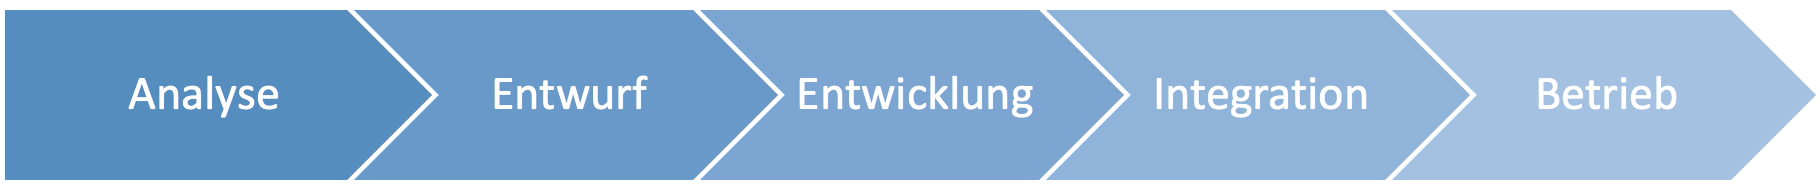
\includegraphics[width=1\textwidth,
		keepaspectratio=true]{bilder/se_phasen.png}
\end{frame}

\begin{frame}
\frametitle{Sequenzielles Modell}
	\begin{itemize}
		\item Softwareentwicklung wird in Aktivitäten (Phasen) gegliedert
		\item Aktivitäten werden sequenziell durchlaufen
		\item Nachfolgeaktivtät kann erst dann starten, wenn der Vorgänger vollständig
		abgeschlossen ist
	\end{itemize}
	\center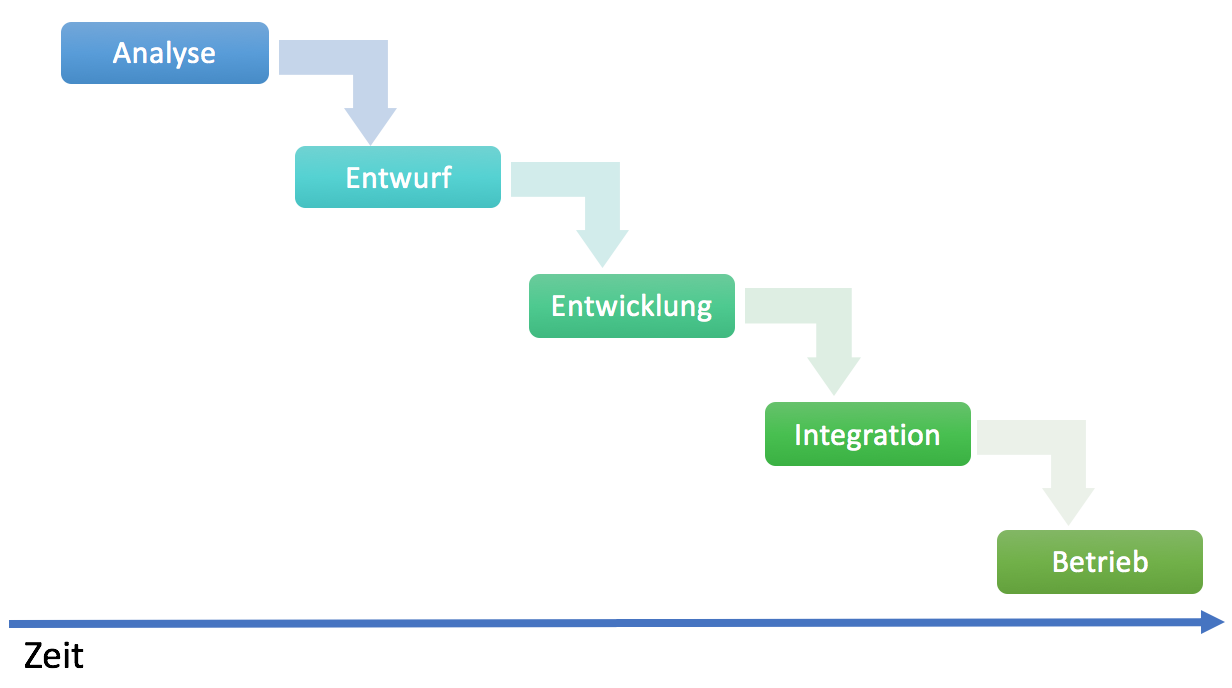
\includegraphics[width=1\textwidth,
		keepaspectratio=true]{bilder/sequenzielles_model.png}
\end{frame}

\begin{frame}
\frametitle{Sequenzielles Modell}
	Vorteile
	\begin{itemize}
		\item leicht verständlich
		\item geringer Managementaufwand
	\end{itemize}
	\bigskip
	Nachteile
	\begin{itemize}
		\item Gesamtdauer = Summe aller Aktivitäten
		\item Fehlende Rückkopplung zwischen den Aktivitäten
		\item Wird ein Problem in Folgeaktivität erkannt
		muss von vorn begonnen werden
		\item Lauffähiges Produkt erst am Ende des Projekts
	\end{itemize}
\end{frame}

\begin{frame}
\frametitle{Wasserfallmodell als bekanntestes sequentielles Modell}
	\begin{itemize}
		\item Sequenzielles Modell mit Rückkopplung
		\item Jede Aktivität wird vollständig ausgeführt
		\item Am Ende jeder Aktivität steht ein Dokumentation
		(Dokumentengetriebenes Modell)
		\item Benutzer nur in der Analyse beteiligt
	\end{itemize}
	\center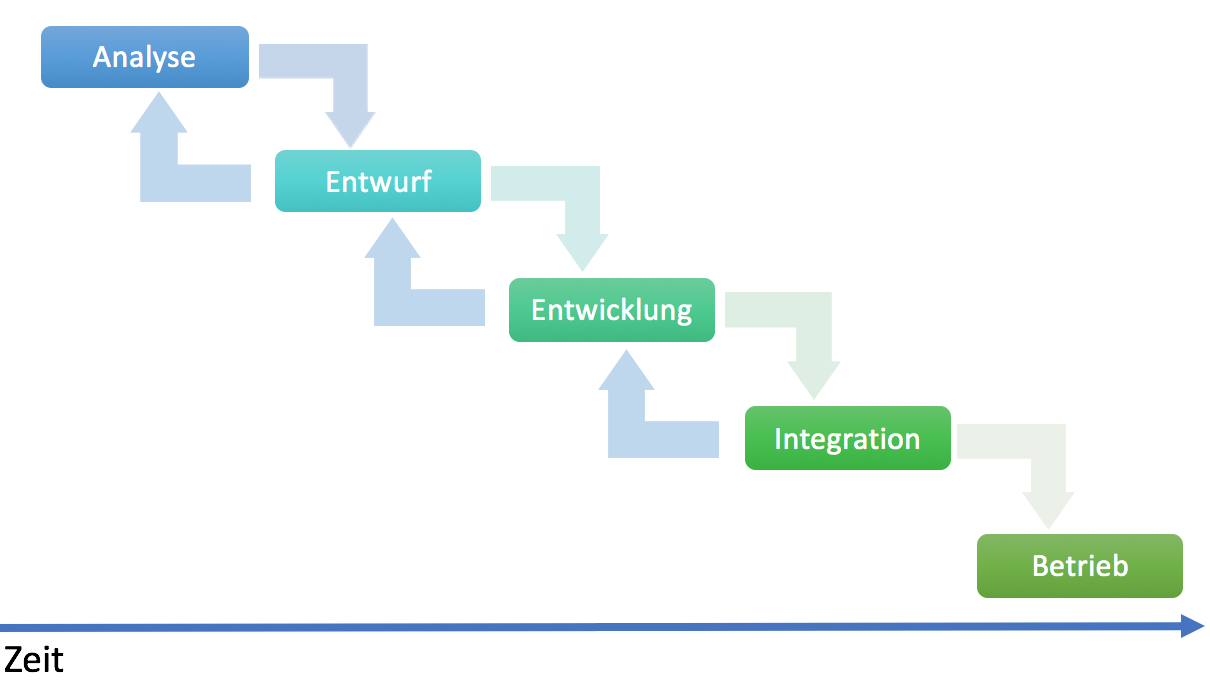
\includegraphics[width=1\textwidth,
		keepaspectratio=true]{bilder/wasserfall_model.png}
\end{frame}

\begin{frame}
\frametitle{Wasserfallmodell als bekanntestes sequentielles Modell}
	Vorteile
	\begin{itemize}
		\item leicht verständlich
		\item geringer Managementaufwand
		\item Aktivitäten gut dokumentiert
	\end{itemize}
	\bigskip
	Nachteile
	\begin{itemize}
		\item Es ist nicht immer sinnvoll alle Aktivitäten vollständig auszuführen
		\item Team ist an die Reihenfolge gebunden
		\item Die Dokumentation kann wichtiger werden als das eigentliche System
		\item Es kann nicht flexibel auf Risikofaktoren reagiert werden
		\item Lauffähiges Produkt erst am Ende des Projekts
	\end{itemize}
\end{frame}

\begin{frame}
\frametitle{Nebenläufiges Modell}
	\begin{itemize}
		\item Durch Überlappungen und Rückkopplungen
		soll die Gesamtzeit reduziert werden
		\item Nachfolger beginnen sobald Vorgänger die ersten
		Informationen bereitgestellt haben
		\item Die Teams arbeiten parallel
		\item Nachfolger müssen auf neue Informationen der Vorgänger reagieren
	\end{itemize}
	\center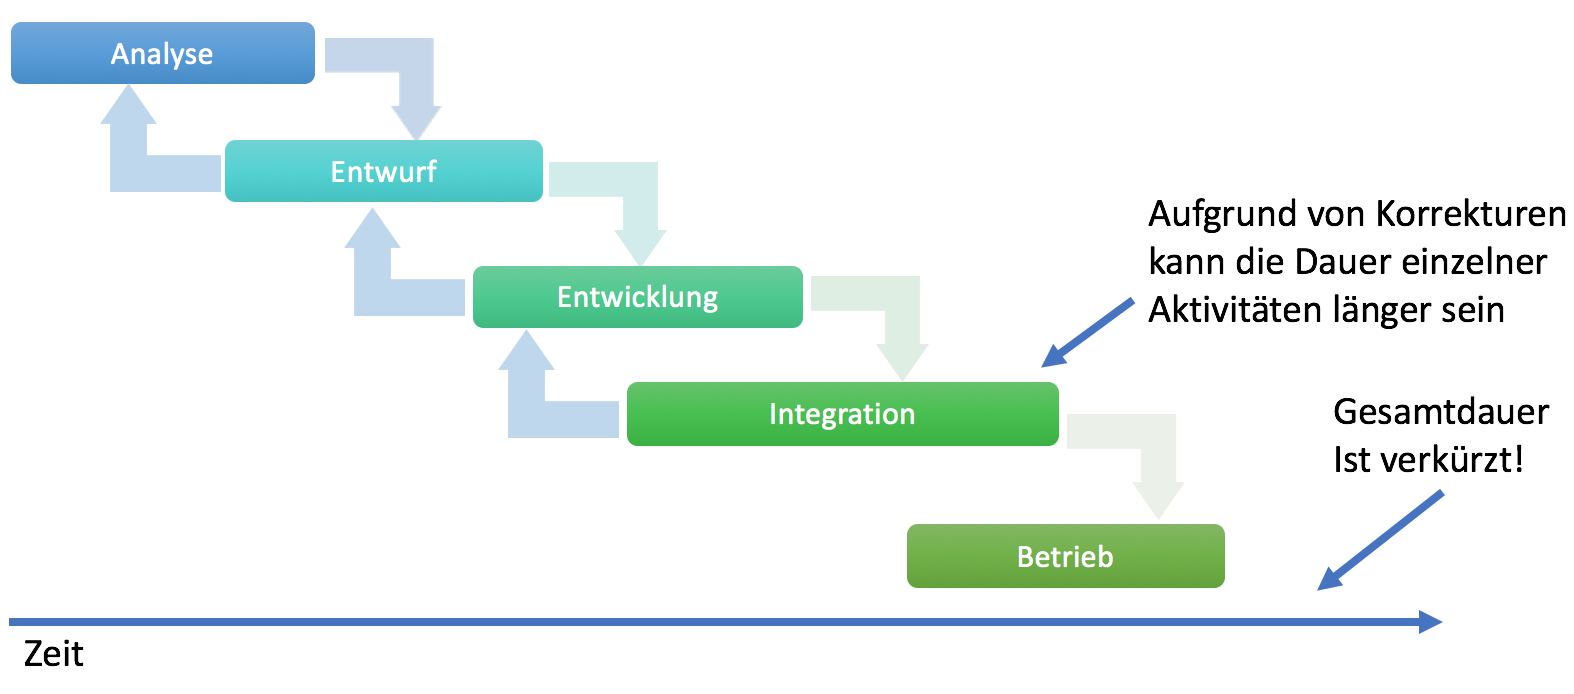
\includegraphics[width=1\textwidth,
		keepaspectratio=true]{bilder/nebenlaufiges_model.png}
\end{frame}

\begin{frame}
\frametitle{Nebenläufiges Modell}
	Vorteile
	\begin{itemize}
		\item Gute Ausnutzung der Zeit
		\item Frühzeitige Rückmeldung möglich
	\end{itemize}
	\bigskip
	Nachteile
	\begin{itemize}
		\item Wichtige Entscheidungen können zu spät getroffen werden
		\item Hoher Planungs- und Personalaufwand
		\item Gefahr dass Nachfolger mit unzureichenden Informationen beginnen
		\item Es kann nicht flexibel auf Risikofaktoren reagiert werden
		\item Kommunikation zwischen den Teams muss aufrecht erhalten werden
	\end{itemize}
\end{frame}

\begin{frame}
\frametitle{Inkrementelles Modell}
	Sequenzielle Modelle
	\begin{itemize}
		\item Bisher wurde in einem Rutsch ein vollständiges Produkt entwickelt
		\item Es wurden vor der Implementierung alle Anforderungen im Detail erarbeitet
		\item Der Kunde ist nur zu Beginn involviert
		\item Es kann mitunter lange dauern bis der Kunde das Produkt nutzen kann
	\end{itemize}
	\bigskip
	Problem
	\begin{itemize}
		\item Zu Beginn sind oftmals nicht alle Anforderungen vorhanden
		\item Der Kunde sollte bereits früh Feedback geben ob das Produkt in seinem
		Sinne entwickelt wurde
	\end{itemize}
\end{frame}

\begin{frame}
\frametitle{Inkrementelles Modell}
	\begin{itemize}
		\item Anforderungen werden vollständig erfasst und modelliert
		\item Produkt wird in Ausbaustufen zerlegt
		\item Jede Ausbaustufe realisiert einen Teil der Funktionalität
		\item Kunde bekommt sehr früh eine erste Version
		\item Erfahrungen fließen in die Folgeversionen mit ein
		\item Jede Version kann in eigenem Projekt entwickelt werden
	\end{itemize}
	\center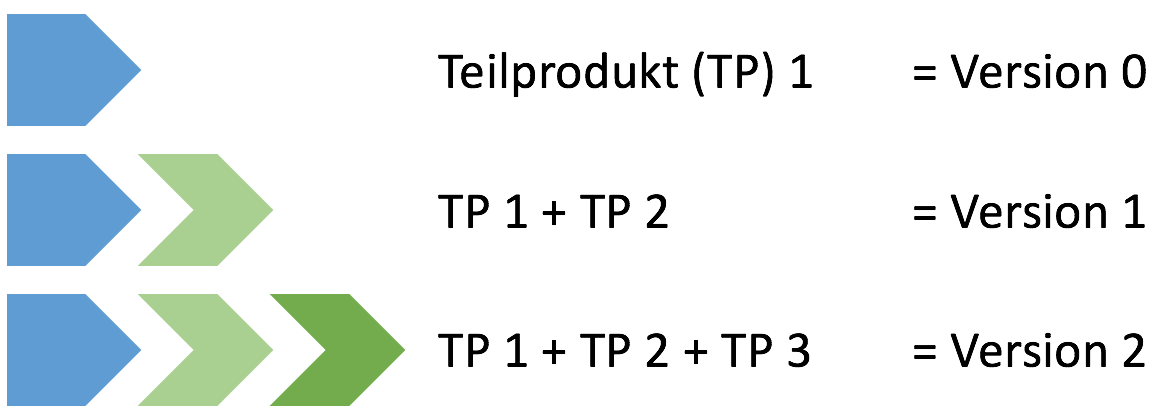
\includegraphics[width=1\textwidth,
		keepaspectratio=true]{bilder/inkrementelles_model.png}
\end{frame}

\begin{frame}
\frametitle{Inkrementelles Modell}
	Vorteile
	\begin{itemize}
		\item Kunde erhält früh und in kurzen Abständen produktionsreife Software
		\item Nicht-Funktionale Anforderungen werden frühzeitig berücksichtigt
		\item Durch vollständige Anforderungen kann die Applikation von
		Beginn an gut strukturiert werden
	\end{itemize}
	\bigskip
	Nachteile
	\begin{itemize}
		\item Vollständige Anforderungen zu Beginn führen zu einer relativ späten
		Auslieferung von Version 0
		\item Modell kann nur verwendet werden, wenn Anforderungen vollständig erfasst
		sind
	\end{itemize}
\end{frame}

\begin{frame}
\frametitle{Evolutionäres Modell}
	\begin{itemize}
		\item Einsatz wenn zu Beginn nicht alle Anforderungen erfasst werden können
		\item Es wird mit Kernanforderungen des Kunden angefangen
		\item Auf dieser Basis wird der Produktkern entwickelt
		\item Kunde kann früh die erste Version einsetzen
		\item Aus den Erfahrungen leitet der Kunde weitere Anforderungen ab
		\item Neue Anforderungen werden in der nächsten Version implementiert
		\item Zyklus aus praktischer Erprobung und Erweiterung + Verbesserung
		\item Software wird in Evolutionsstufen entwickelt
		\item Grundlage der agilen Prozessmodelle
	\end{itemize}
\end{frame}

\begin{frame}
\frametitle{Evolutionäres Modell}
	Vorteile
	\begin{itemize}
		\item Anforderungen müssen zu Beginn nicht vollständig vorliegen
		\item Kunde kann sehr früh die erste Version einsetzen und bewerten
		\item Erfahrungen aus Produktiveinsatz können in nächste Version einfließen
		\item Durch kurze Entwicklungszyklen kann kurzzeitig auf Änderungen reagiert werden
	\end{itemize}
	\bigskip
	Nachteile
	\begin{itemize}
		\item Gefahr dass bei Folgeversionen die gesamte Architektur überarbeitet werden muss
		\item Es besteht die Gefahr dass ``evolutionär'' nur ein Vorwand für mangelhafte
		Spezifikation ist
	\end{itemize}
\end{frame}

\begin{frame}
\frametitle{Übung 2.2}
	Wann würden Sie evolutionäre Modelle anwenden und wann sequenzielle?
\end{frame}

\begin{frame}
\frametitle{Anwendung evolutionärer Modelle}
	\begin{itemize}
		\item Bei Projekten mit offenen Fragen (bzgl. Technologie, Domäne, \ldots)
		\item Bei Projekten mit unklaren oder sich ändernden Anforderungen
		\item Bei sehr komplexen Projekten
	\end{itemize}
\end{frame}

\begin{frame}
\frametitle{Übung 2.3}
	Entwickeln Sie eine Applikation. Für Analyse, Entwurf und Entwicklung benötigen
	Sie jeweils 2 Monate. Sie führen eine nebenläufige Entwicklung durch. Dabei wird
	jeweils 75\% der Vorgängerpahse überlappt. Aufgrund des Kommunikations- und
	Änderungsaufwands verlängern sich die Phasen Entwurf und Entwicklung um jeweils 20\%.
	Wie viel Zeit sparen Sie durch die Nebenläufige Entwicklung ein?
\end{frame}

\ifloesung
\begin{frame}
\frametitle{Übung 2.3 - Lösung}
	Sequenziell = 2M A + 2M E + 2M C = 6 Monate
	\newline
	Nebenläufig = 2M A + 2.4M E (Start 0.5) + 2.4M C (Start 1) = ca. 3.5 Monate
\end{frame}
\fi

\begin{frame}
\frametitle{Übung 2.4}
	Sie arbeiten nun nach dem inkrementellen Vorgehensmodell. Die Analyse benötigt 2 Monate. Sie
	entwicklen 2 inkremente (V1 und V2). Für jedes Inkrement benötigen Entwurf und Entwicklung jeweils
	1 Monat. Wie viel Zeit wird benötigt um V1, V2 sowie die finale Applikation fertig zu stellen?
	Wo liegt der Vorteil im Vergleich zur sequenziellen Entwicklung?
\end{frame}

\ifloesung
\begin{frame}
\frametitle{Übung 2.4 - Lösung}
	V1 = 2M A + 1M E + 1M C = 4 Monate
	\newline
	V2 = 1M E + 1M C = 2 Monate
	\newline
	V3 = V1 + V2 = 6 Monate
	\newline\newline
	Vorteile
	\begin{itemize}
		\item Kunde kann Applikation bereits nach 4 Monaten nutzen
		\item Inkremente können jeweils in eigenen Projekten realisiert werden
		\item \ldots
	\end{itemize}
\end{frame}
\fi

\begin{frame}
\frametitle{Übung 2.5}
	Entwickeln Sie eine Applikation nun nach dem evolutionären Vorgehensmodell. Für Analyse,
	Entwurf und Entwicklung benötigen Sie jeweils 1 Monat. Sie entwickeln 2 Versionen (V1 und V2).
	Wie lange dauert die Entwicklungszeit für V1 und V2 sowie für das ganze Produkt?
	Wo liegt der Vorteil im Vergleich zur sequenziellen Entwicklung?
\end{frame}

\ifloesung
\begin{frame}[fragile]
\frametitle{Übung 2.5 - Lösung}
	V1 = 1M A + 1M E + 1M C = 3 Monate
	\newline
	V2 = 1M A + 1M E + 1M C = 3 Monate
	\newline
	V3 = V1 + V2 = 6 Monate
	\newline\newline
	Vorteile
	\begin{itemize}
		\item Kunde kann Applikation bereits nach 3 Monaten nutzen
		\item Architektur und Code ist auf die Problemstellung abgestimmt
		\item \ldots
	\end{itemize}
\end{frame}
\fi

\begin{frame}
\frametitle{Prototyping Modell}
	\begin{itemize}
		\item Entwicklung einer Anfangsimplementierung
		\item Benutzer geben zu dieser (konkreten) Implementierung Feedback
		\item Äußerungen der Benutzer werden in neuer Version des Systems berücksichtigt
		\item Die Schritte 2 – 3 werden solange durchgeführt bis ein angemessenes System entstanden ist
	\end{itemize}
	\begin{block}{Prototyp}
		Provisorisches Softwaresystem (Modell), das erstellt wird,
		um Anforderungen zu klären oder zu veranschaulichen.
	\end{block}
\end{frame}

\begin{frame}
\frametitle{Prototyping Modell}
	\begin{block}{Prototyping}
		Folge von Prototypen, die bestimmte Systemfunktionen oder -aspekte
		frühzeitig realisieren oder vortäuschen, so dass der Benutzer:
		\begin{itemize}
			\item den gewünschten Eindruck erhält
			\item sich mit dem Prototyp auseinandersetzen kann.
		\end{itemize}
	\end{block}
	\begin{block}{Rapid Prototyping}
		Art von Prototyping bei dem der Fokus auf der Entwicklung
		von Prototypen zu Beginn des Softwareprozesses an liegt,
		um so möglichst von Anfang an Feedback vom Nutzer einzuholen.
	\end{block}
\end{frame}

\begin{frame}
\frametitle{Prototyping Modell - Arten von Prototypen}
	Prototypen haben die folgene Verwendung:
	\begin{itemize}
		\item Klärung von Anforderungen oder Entwicklungsproblemen
		\item Durchführung von Experimenten und Sammlung von Erfahrungen
	\end{itemize}
	\bigskip
	Dabei wird zwischen verschiedenen Arten von Prototypen unterschieden.
\end{frame}

\begin{frame}
\frametitle{Prototyping Modell - Arten von Prototypen}
	Demonstrationsprototyp
	\begin{itemize}
		\item Dient der Auftragsakquisition
		\item Auftraggeber bekommt ersten Eindruck vom Produkt
		\item Schnelle Entwicklung in frühem Stadium des Entwicklungsprozesses
		\item Auf Standards und Best Practices bei der Entwicklung wird verzichtet
		\item Wegwerfprodukt
	\end{itemize}
\end{frame}

\begin{frame}
\frametitle{Prototyping Modell - Arten von Prototypen}
	Funktionaler Prototyp
	\begin{itemize}
		\item Unterstützt die Anforderungsanalyse
		\item Modelliert Ausschnitte der Bedienoberfläche und/oder Teile der Funktionalität
		\item Kann in Architektur bereits dem Zielsystem entsprechen
		\item Dient dem Nachweis der technischen Machbarkeit
		\item Auch für Benutzerfeedback hinsichtlich Software-Ergonomie
	\end{itemize}
\end{frame}

\begin{frame}
\frametitle{Prototyping Modell - Arten von Prototypen}
	Labormuster
	\begin{itemize}
		\item Modelliert technische Aspekte des Zielsystems
		\item Experimentiersystem für Entwickler
		\item Für Machbarkeitsstudien
		\item In der Regel sind Endnutzer nicht an der Evaluation beteiligt
	\end{itemize}
	\bigskip
	Pilotsystem
	\begin{itemize}
		\item Realisiert einen abgeschlossenen Bereich des Zielsystems
		\item Funktionalität und Qualität reichen mindestens für vorübergehenden
		Produktiveinsatz
		\item Wird Schrittweise erweitert
	\end{itemize}
\end{frame}

\begin{frame}
\frametitle{Prototyping Modell - Arten von Prototypen}
	Ein Softwaresystem besteht in der Regel aus verschiedenen Komponenten/Schichten.
	Aus diesem Grund lassen sich Prototypen auch in horizontale oder vertikale
	Prototypen unterscheiden.
	\begin{itemize}
		\item Horizontale Prototypen realisieren nur eine Schicht des Systems
		(beispielsweise Nutzeroberfläche oder Datenbankschicht)
		\item Vertikale Prototypen implementieren einen funktionalen Teilbereich
		durch alle Schichten hindurch (End-2-End)
	\end{itemize}
\end{frame}

\begin{frame}
\frametitle{Prototyping Modell - Arten von Prototypen}
	\center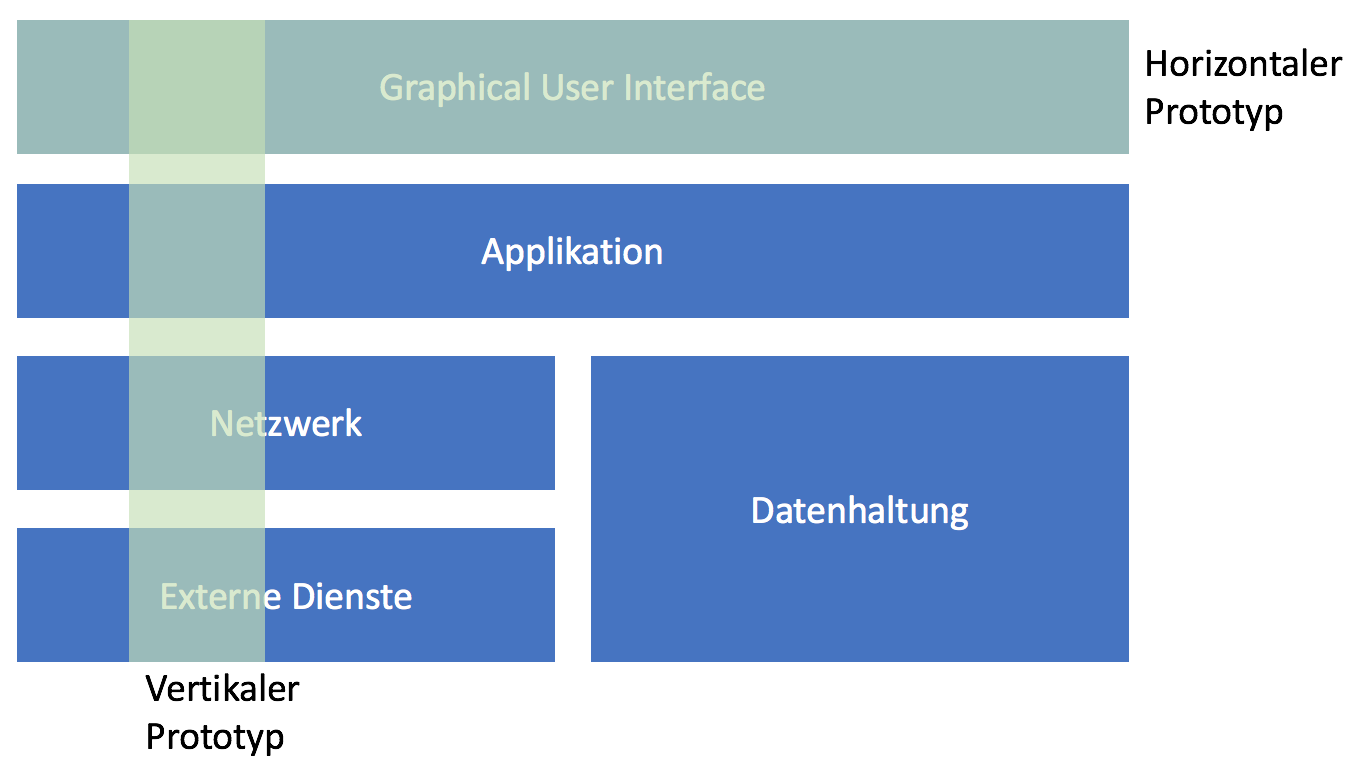
\includegraphics[width=1\textwidth,
			keepaspectratio=true]{bilder/prototypen.png}
\end{frame}

\begin{frame}
\frametitle{Prototyping Modell - Prozess}
	\center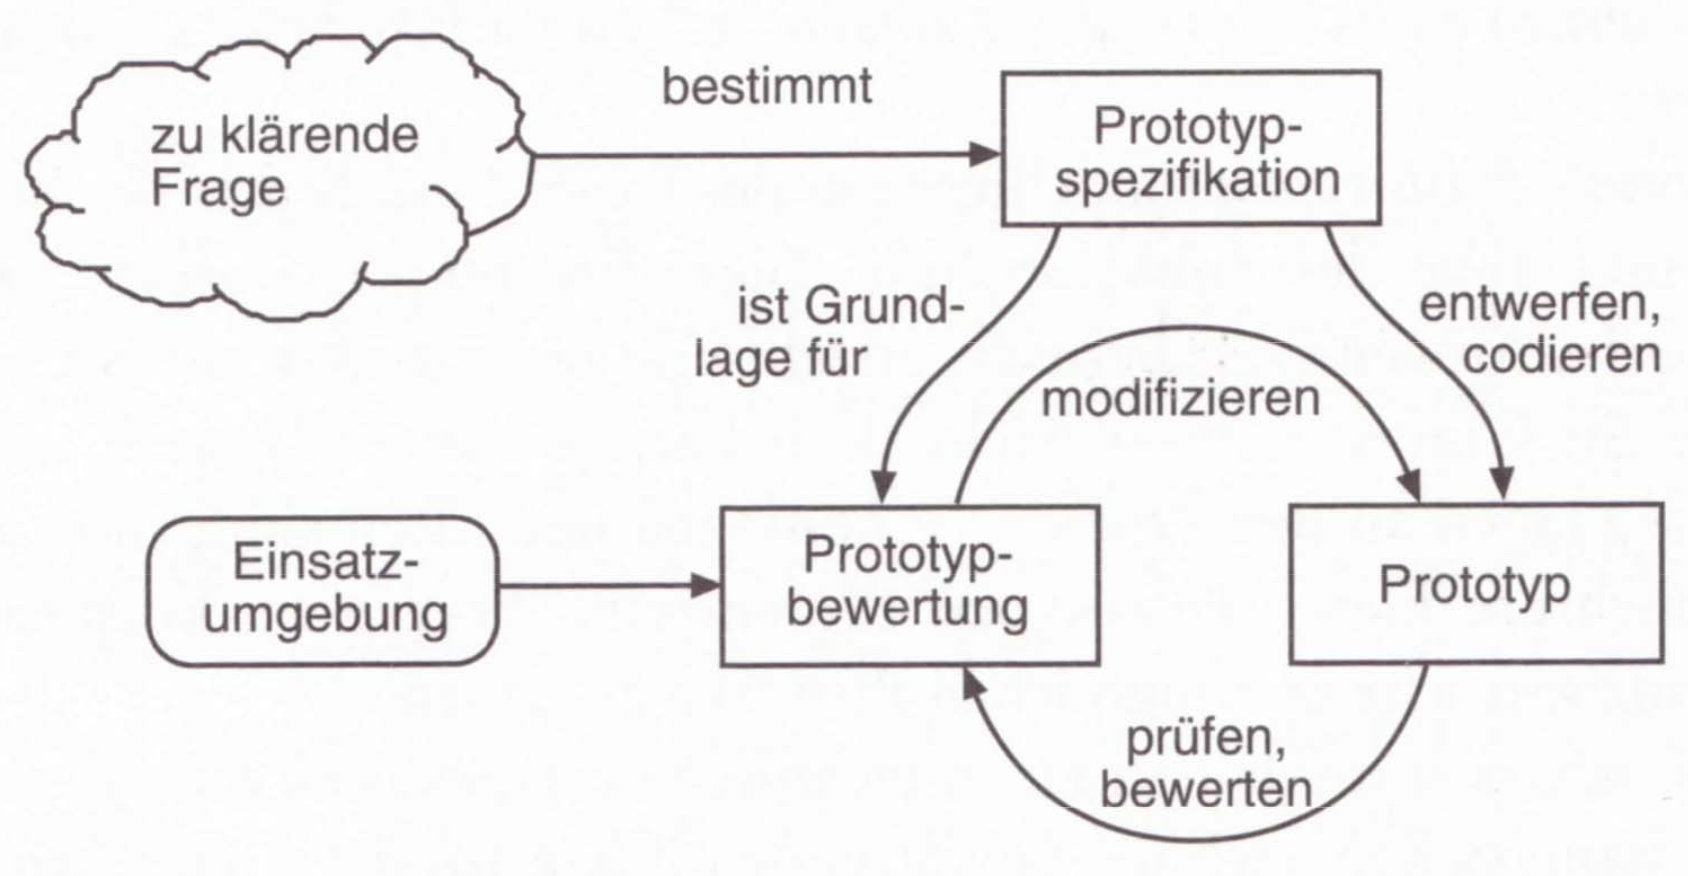
\includegraphics[width=1\textwidth,
			keepaspectratio=true]{bilder/prototyp_entwicklung.png}
\end{frame}

\begin{frame}
\frametitle{Prototyping Modell - Anwendbarkeit}
	\begin{itemize}
		\item Für sehr interaktive Systeme
		\item Für kleine/mittlere oder Teile großer Systeme
		\item Für Systeme mit kurzer Lebensdauer
		\item Für Systeme, die schlecht vorab planbar sind
	\end{itemize}
	\bigskip
	Prototyping wird selten als alleinstehendes Vorgehensmodell verwendet.
	Vielmehr findet es im Rahmen anderer Vorgehensmodelle statt.
\end{frame}

\begin{frame}
\frametitle{Übung 2.6}
	Welche Vor- und Nachteile hat die Verwendung von Prototypen?
\end{frame}

\begin{frame}
\frametitle{Prototyping Modell}
	Vorteile
	\begin{itemize}
		\item Reduziert das Entwicklungsrisiko
		\item Missverständnisse in den Anforderungen fallen frühzeitig auf
		\item Fehlende Anforderungen werden identifiziert wodurch die Planung optimiert wird
		\item Fördert die Kreativität
	\end{itemize}
	\bigskip
	Nachteile
	\begin{itemize}
		\item Die enstehenden Applikationen sind oftmals schlechter strukturiert
		\item Wegwerf-Prototypen werden of nachträglich als evolutionär entwickeltes System deklariert
		und produktiv eingesetzt
	\end{itemize}
\end{frame}

\begin{frame}
\frametitle{Spiralmodell}
	\begin{itemize}
		\item Generisches Vorgehensmodell
		\item Bietet Anleitung um unter Berücksichtigung von spezifischen Risikofaktoren
		ein auf das Projekt zugeschnittenes Vorgehensmodell zu entwickeln
		\item Mit Blick auf die Risiken wird für jede Phase ein eigenes Vorgehensmodell
		verwendet
	\end{itemize}
\end{frame}

\begin{frame}
\frametitle{Spiralmodell}
	Für jede Phase werden 4 Schritte durchlaufen.
	\newline\newline
	Schritt 1:
	\begin{enumerate}
		\item Identifikation der Ziele des Teilprodukts (Leistung, Funktionalität...)
		\item Alternative Möglichkeiten Aufzeigen um das Teilprodukt zu realisieren
		(Entwurf 1, Entwurf 2, Kauf, Wiederverwendung)
		\item Randbedingungen beachten (Schnittstellen, Zeit, Budget ...)
	\end{enumerate}
\end{frame}

\begin{frame}
\frametitle{Spiralmodell}
	Schritt 2:
	\begin{enumerate}
		\item Alternativen evaluieren
		\item Risiken identifizieren
		\item Zeichnen sich Risiken ab, werden geeignete Maßnahmen ergriffen
		um sie zu vermeiden
		\item Prototypen entwickeln
	\end{enumerate}
	\bigskip
	Schritt 3:
	\begin{enumerate}
		\item Unter Berücksichtigung der verbleibenden Risiken wird geeignetes
		Vorgehensmodell gewählt
		\item Entwicklung
	\end{enumerate}
	\bigskip
	Schritt 4:
	\begin{enumerate}
		\item Nächsten Zyklus planen
		\item Review der vorhergehenden Schritte
	\end{enumerate}
\end{frame}

\begin{frame}
\frametitle{Spiralmodell}
	\center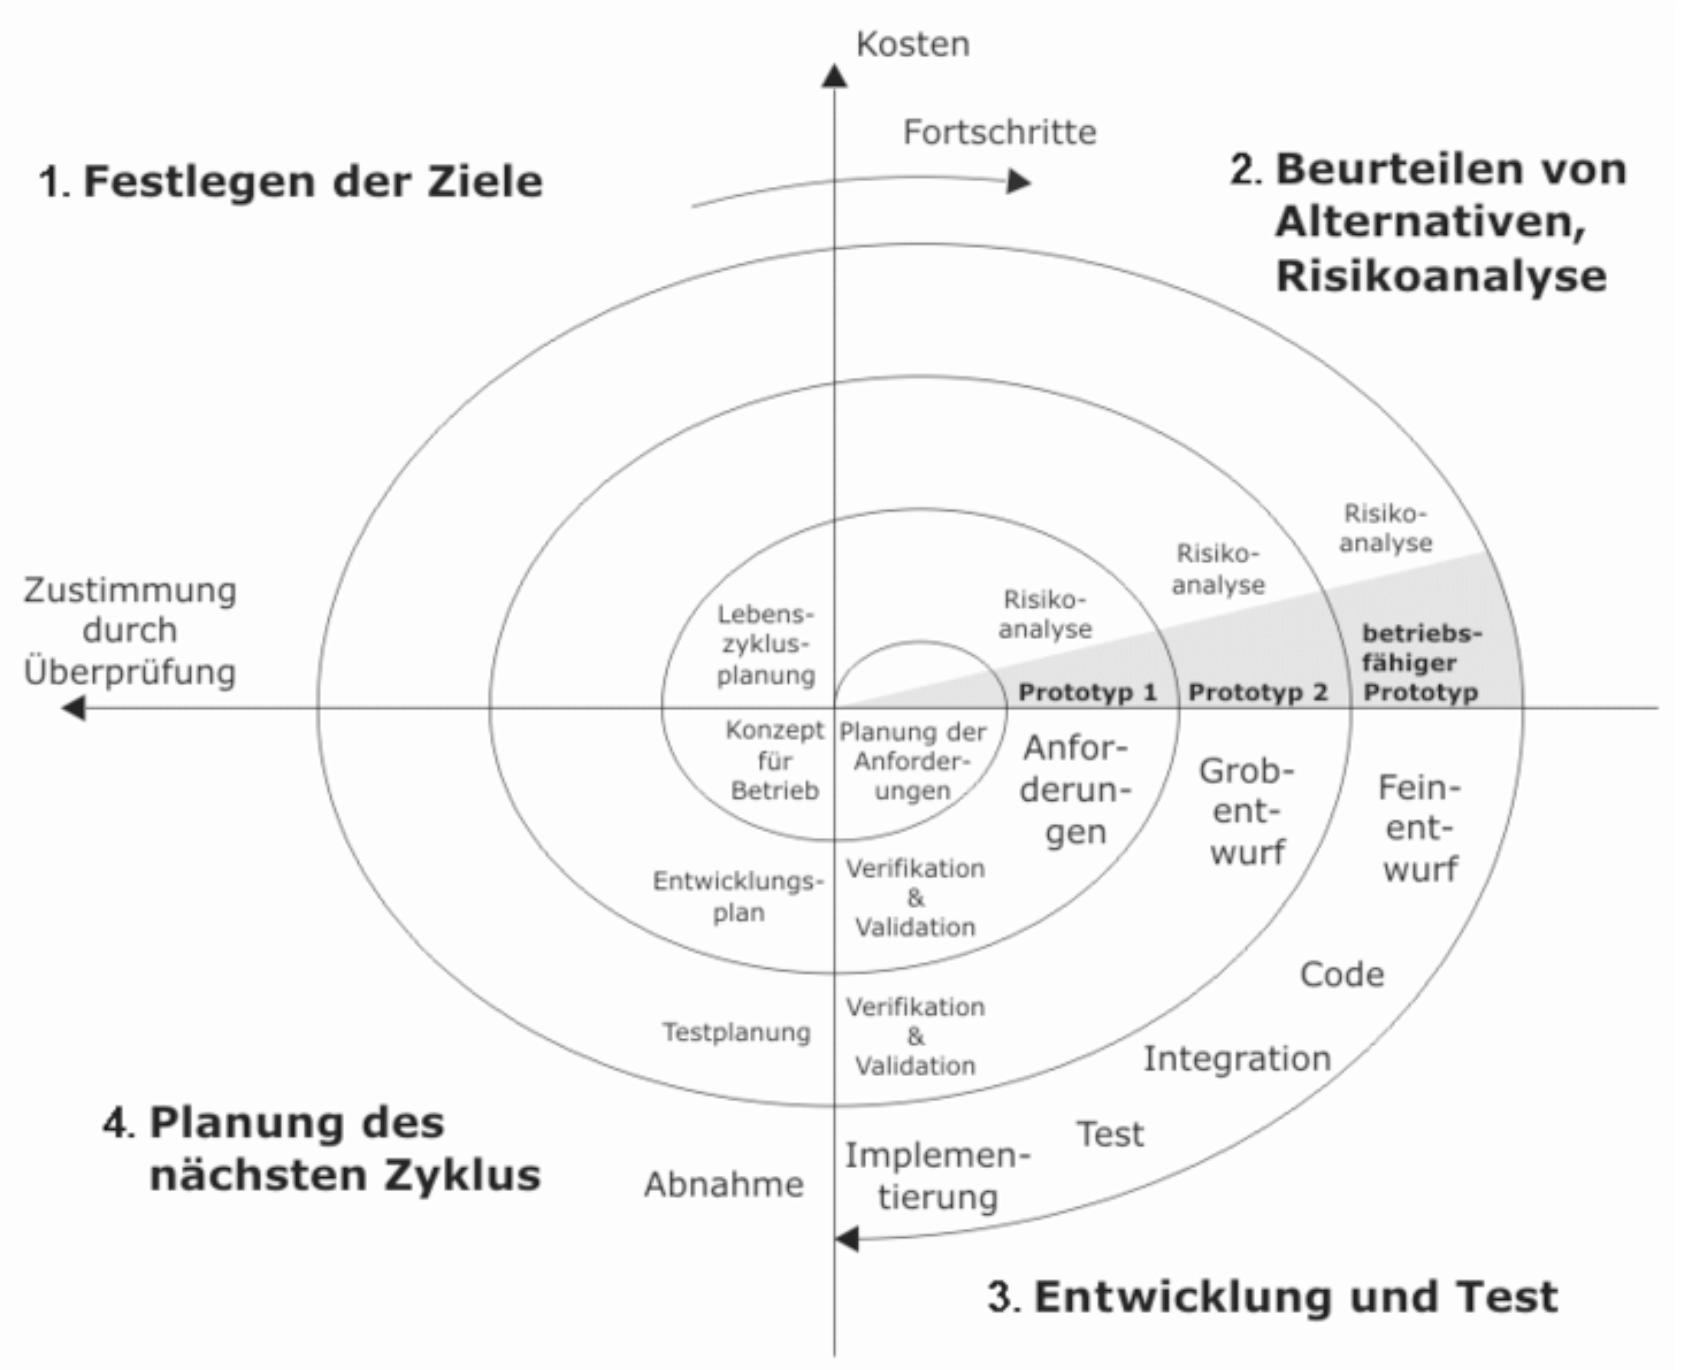
\includegraphics[width=1\textwidth,
			keepaspectratio=true]{bilder/spiralmodell.png}
\end{frame}

\begin{frame}
\frametitle{Spiralmodell}
	\begin{itemize}
		\item Fläche der Spirale steht für angefallene Kosten
		\item Winkel der Spirale zeigt Fortschritt der Entwicklung im aktuellen Durchlauf
	\end{itemize}
\end{frame}

\begin{frame}
\frametitle{Spiralmodell}
	Vorteile
	\begin{itemize}
		\item Risiken frühzeitig berücksichtigt
		\item Modell ist sehr flexibel
		\item Andere Vorgehensmodelle können integriert werden
		\item Frühe Erkennung und Eliminierung von Fehlern
		\item Unterstützt Wiederverwendung da Alternativen berücksichtigt werden
		\item Anpassung der Entwicklung durch Erfahrungen die im Zyklus t-1 gewonnen wurden
	\end{itemize}
\end{frame}

\begin{frame}
\frametitle{Spiralmodell}
	Nachteile
	\begin{itemize}
	\item Ständiger Wechsel des Vorgehensmodells ist wenig Praktikabel
			\begin{itemize}
				\item hoher Managementaufwand
				\item Mitarbeiter müssen sehr flexibel seinem
				\item Detailwissen und Erfahrung verschiedener Modelle sind Voraussetzung
				\item Nicht für kleine bis mittlere Projekte geeignet
				\item Oftmals fehlende Erfahrung im Risikomanagement
				\item Geplant wird über einen Zyklus, End-2-End Planung nicht möglich
			\end{itemize}
	\end{itemize}
\end{frame}

\begin{frame}
\frametitle{Übung 2.7}
	Nennen Sie 5 mögliche Gründe warum Projekte (insbesondere Softwareprojekte) scheitern.
\end{frame}

\ifloesung
\begin{frame}[fragile]
\frametitle{Übung 2.7 - Lösung}
	\begin{itemize}
		\item Projektziel/Strategie nicht klar kommuniziert oder gar definiert
		\item Verwendung unausgereifte Technologien
		\item Kommunikationsdefizite innerhalb des Teams
		\item Kommunikationsdefizite gegenüber dem Kunden
		\item Kein klares Projektvorgehen definiert
		\item Fehlende Transparenz bezüglich des Projektfortschritts
		\item Schlechte Verteilung von Skills und Erfahrung
		\item Unternehmenspolitische Hürden
		\item \ldots
	\end{itemize}
\end{frame}
\fi

\begin{frame}
\frametitle{Übung 2.8}
	In einem Softwareprojekt können immer wieder Führungsprobleme auftreten.
	Was können mögliche Ursachen dafür sein? Betrachten Sie die Frage aus dem
	Blickwinkel des Projektleiters sowie aus Perspektive des Mitarbeiters.
\end{frame}

\ifloesung
\begin{frame}[fragile]
\frametitle{Übung 2.8 - Lösung}
	Sicht des Projektleiters
	\begin{itemize}
		\item Fortschritte werden nicht korrekt Kommuniziert / Fehlende Transparenz
		\item Komplexität einzelner Arbeitspakete für Nicht-Entwickler schwer
		bewertbar
		\item Fehlender Fokus der Entwickler
		\item Projektressourcen werden abgezogen
		\item \ldots
	\end{itemize}
	\bigskip
	Sicht des Mitarbeiter
	\begin{itemize}
		\item PM bringt zu wenig technisches Wissen mit
		\item Auswirkungen von ad-hoc Änderungen werden vom Management oft
		unterschätzt / PM hat kein Durchsetzungsvermögen
		\item \ldots
	\end{itemize}
\end{frame}
\fi

\subsection{Monumentale Prozessmodelle}
\begin{frame}
\frametitle{Monumentale Prozessmodelle}
\huge Monumentale Prozessmodelle
\end{frame}

\begin{frame}
\frametitle{Monumentale Prozessmodelle}
	\begin{block}{Definition Prozessmodell}
		Während Vorgehensmodelle den Kern bilden, ergänzen Prozessmodelle die Vorgehensmodelle um
		Organisationsstrukturen für Projektmanagement, Qualitätssicherung, Dokumentation sowie
		Konfigurationsverwaltung.
	\end{block}
	\bigskip
	\begin{block}{Monumental}
		\begin{itemize}
			\item Prozessmodelle mit sehr umfangreicher Beschreibung
			\item Dokumentation von zentraler Bedeutung und umfangreich
			\item Planung ist fest vorgegeben
		\end{itemize}
  \end{block}
\end{frame}

\begin{frame}
\frametitle{Monumentale Prozessmodelle}
	\begin{itemize}
		\item Aktivitäten werden von Mitarbeitern durchgeführt
		\item Die Kenntnisse/Fähgikeiten die als Vorraussetzung dienen
		werden durch Rollen beschrieben
		\item Die Durchführung wird genauer spezifiziert
		\begin{itemize}
			\item Weitere durchzuführende Aktivität?
			\item Rollenzuordnung
			\item Zu verwendende Artifakte
			\item Zu erstellende Artifakte
			\item Zu beachtende Konventionen, Methoden, Richtlinien
			\item Einzusetzende Werkzeuge
		\end{itemize}
	\end{itemize}
\end{frame}

\begin{frame}
\frametitle{Monumentale Prozessmodelle}
	\center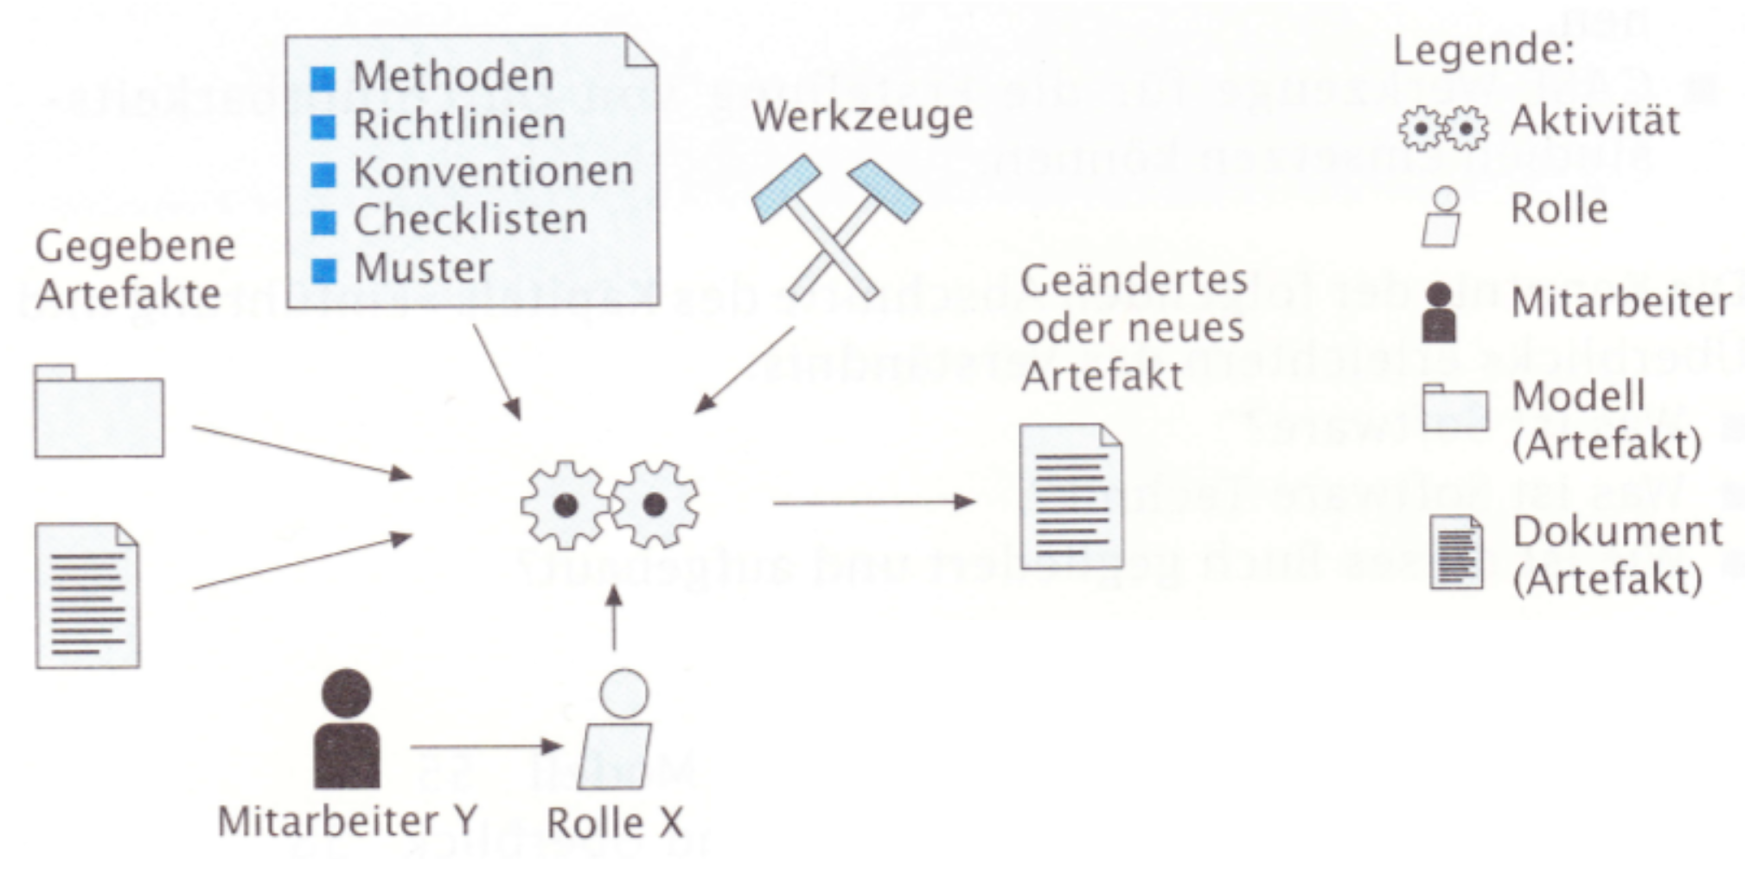
\includegraphics[width=1\textwidth,
			keepaspectratio=true]{bilder/prozessmodell.png}
\end{frame}

\begin{frame}
\frametitle{V-Modell}
	\begin{itemize}
		\item Erweiterung des Wasserfallmodells
		\item Integration einer Qualitätssicherung
		\item Erzeugte Teilprodukte werden Verifikation und Validierung unterzogen
		\begin{itemize}
			\item Verifikation: Prüfung ob das SW-Produkt mit der Spezifikation
			übereinstimmt (``Am I building the product right?'')
			\item Validierung: Eignung des Produkts für den vorgeschriebenen
			Einsatzzweck (``Am I building the right product?'')
		\end{itemize}
	\end{itemize}
\end{frame}

\begin{frame}
\frametitle{V-Modell}
	\center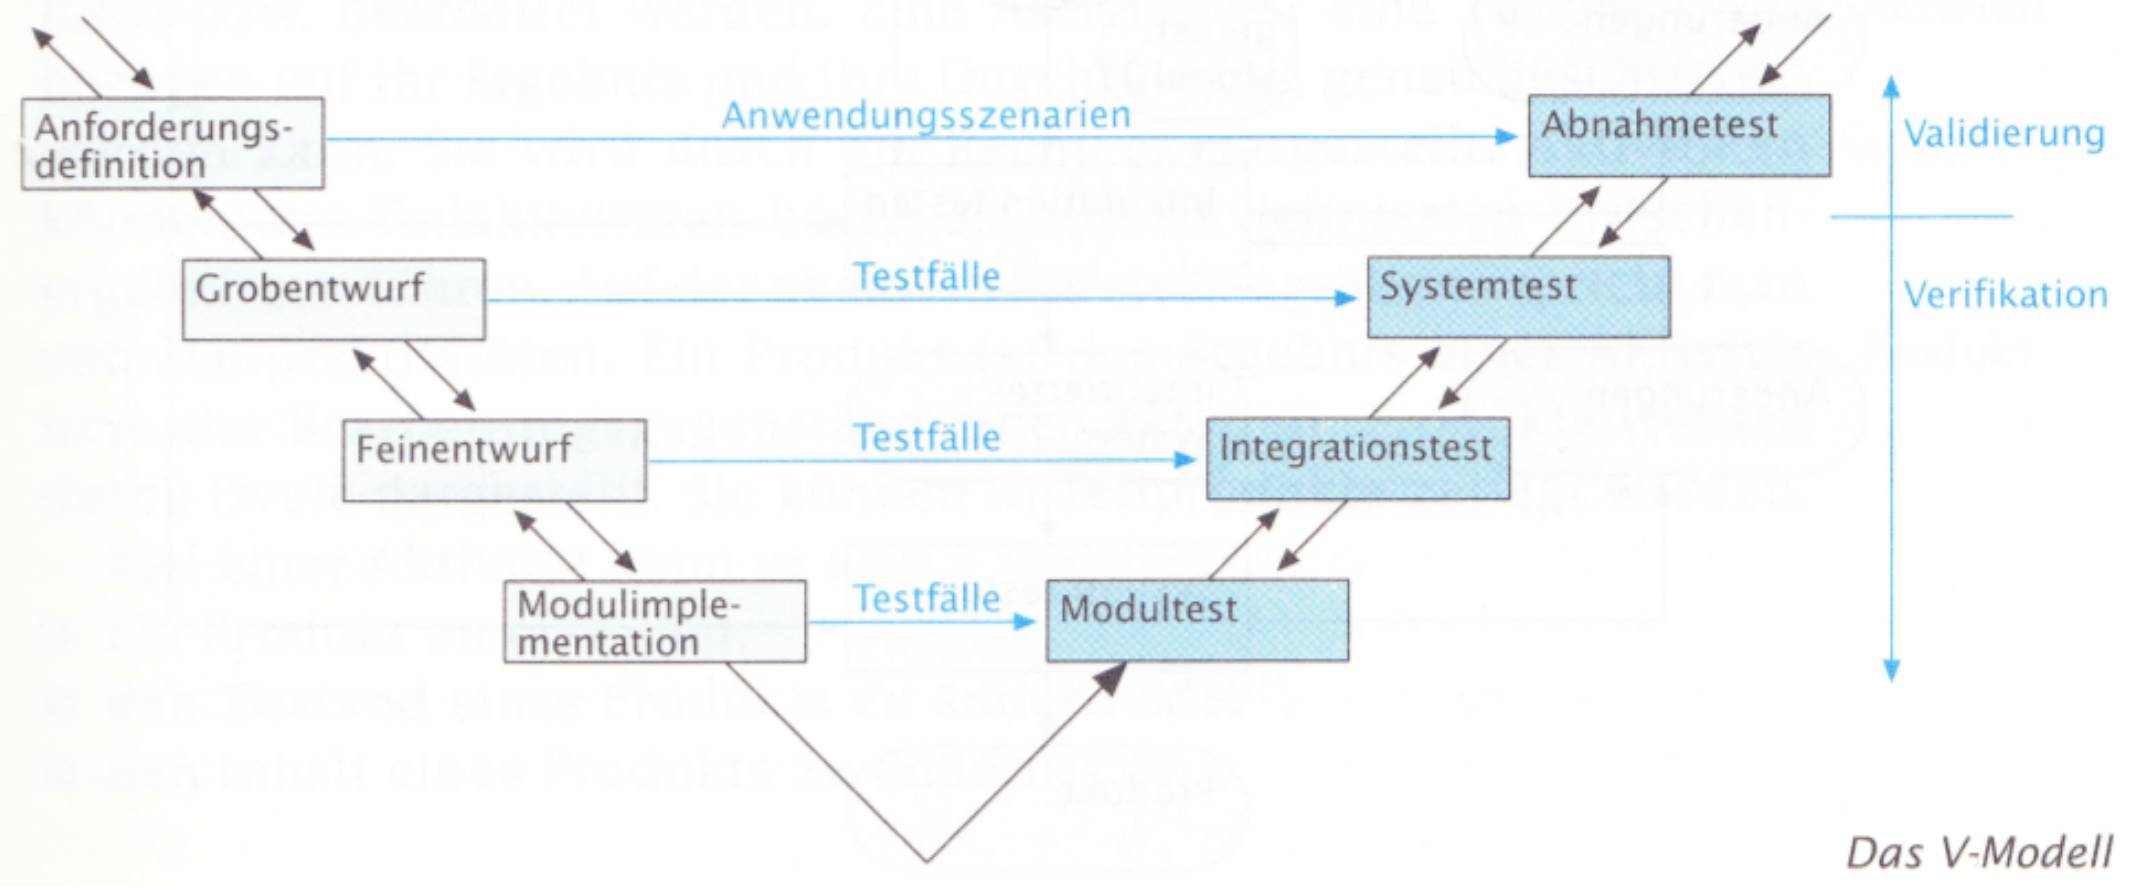
\includegraphics[width=1\textwidth,
			keepaspectratio=true]{bilder/vmodell.png}
\end{frame}

\begin{frame}
\frametitle{V-Modell Xtreme Tailoring}
	\begin{itemize}
		\item Regelt ``wer'', ``wann'', ``was'' in einem Projekt zu tun hat
		\item Unterscheided 4 verschiedene Projekttypen zur Abbildung von
		Auftraggeber und Auftragnehmer
		\item Charakteristische Projekteigenschaften werden berücksichtigt
	\end{itemize}
	\center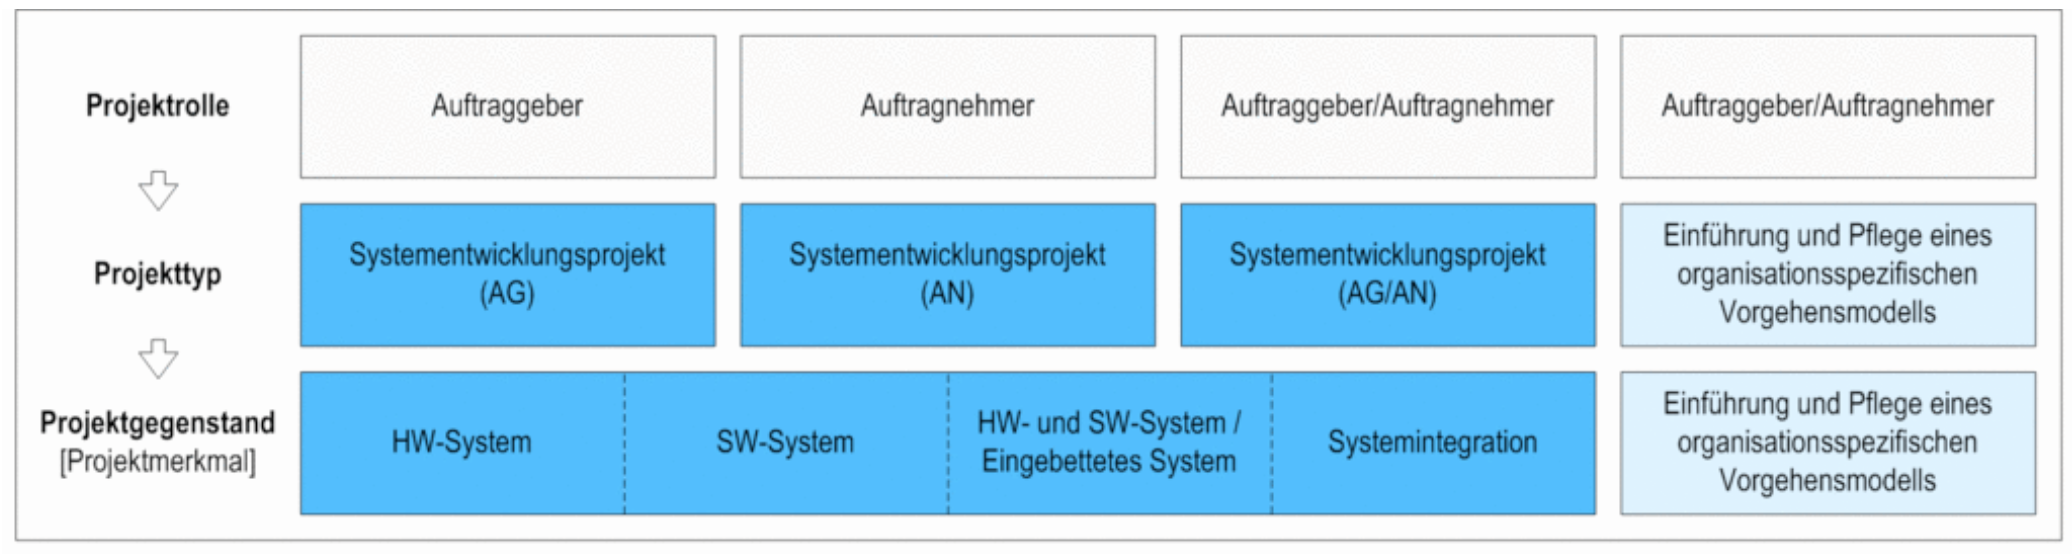
\includegraphics[width=1\textwidth,
			keepaspectratio=true]{bilder/vmodell_typen.png}
\end{frame}

\begin{frame}
\frametitle{V-Modell Xtreme Tailoring}
	\begin{itemize}
		\item Für jeden Typen bietet V-Modell angepasste Varianten an
		\item Variante bestimmt dann die Durchführungsstrategie
	\end{itemize}
	\center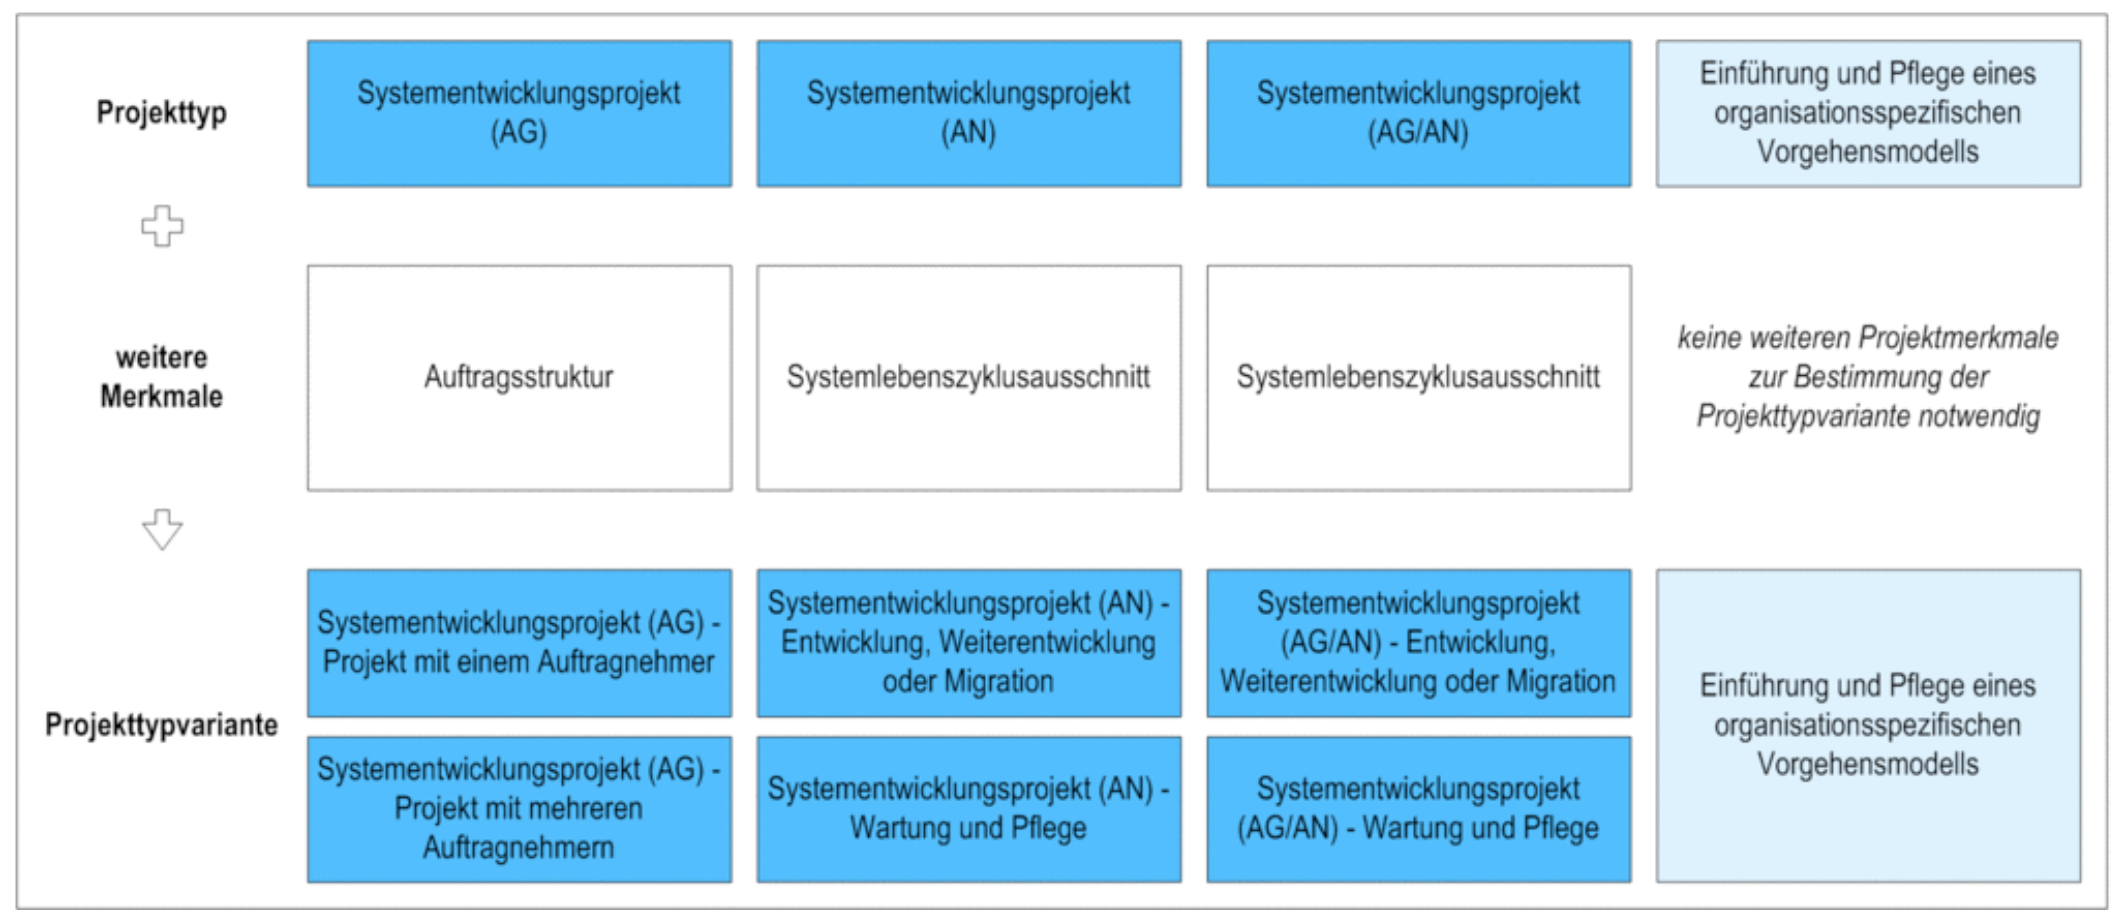
\includegraphics[width=1\textwidth,
			keepaspectratio=true]{bilder/vmodell_typen_varianten.png}
\end{frame}

\begin{frame}
\frametitle{V-Modell Xtreme Tailoring}
	\begin{itemize}
		\item Projektdurchführungsstrategie legt Reihenfolge der zu erstellenden
		Produkte und durchzuführenden Aktivitäten fest
		\item Grundlage für den Projektplan
		\item Es stehen 11 Strategien zur Auswahl
	\end{itemize}
	\bigskip
	Für Entwicklungsprozess aus AN-Sicht mit hohem Realisierungsrisiko werden
	z.B. folgende Strategien vorgeschlagen:
	\begin{itemize}
		\item Inkrementelle Entwicklung
		\item Komponentenbasierte Entwicklung
		\item Agile Entwicklung
		\item \ldots
	\end{itemize}
\end{frame}

\begin{frame}
\frametitle{V-Modell Xtreme Tailoring}
	\begin{itemize}
		\item Produkte sind Ergebnisse und Zwischenergebnisse eines Projekts
		\item 4 Produkte werden für alle Projekte verpflichtend vorgeschlagen:
		\begin{itemize}
			\item Projekthandbuch
			\item Projektplan
			\item QS-Handbuch
			\item Produktbibliothek
		\end{itemize}
		\item Jedes Produkt wird durch eine Aktivität erstellt
	\end{itemize}
\end{frame}

\begin{frame}
\frametitle{V-Modell Xtreme Tailoring}
	\begin{itemize}
		\item Zusammengehörige Produkte und Aktivitäten werden als Disziplinen
		bezeichnet
		\item Es werden 13 Disziplinen unterschieden und in die drei Bereiche
		Projekt, Entwicklung und Organisation unterteilt
	\end{itemize}
	\center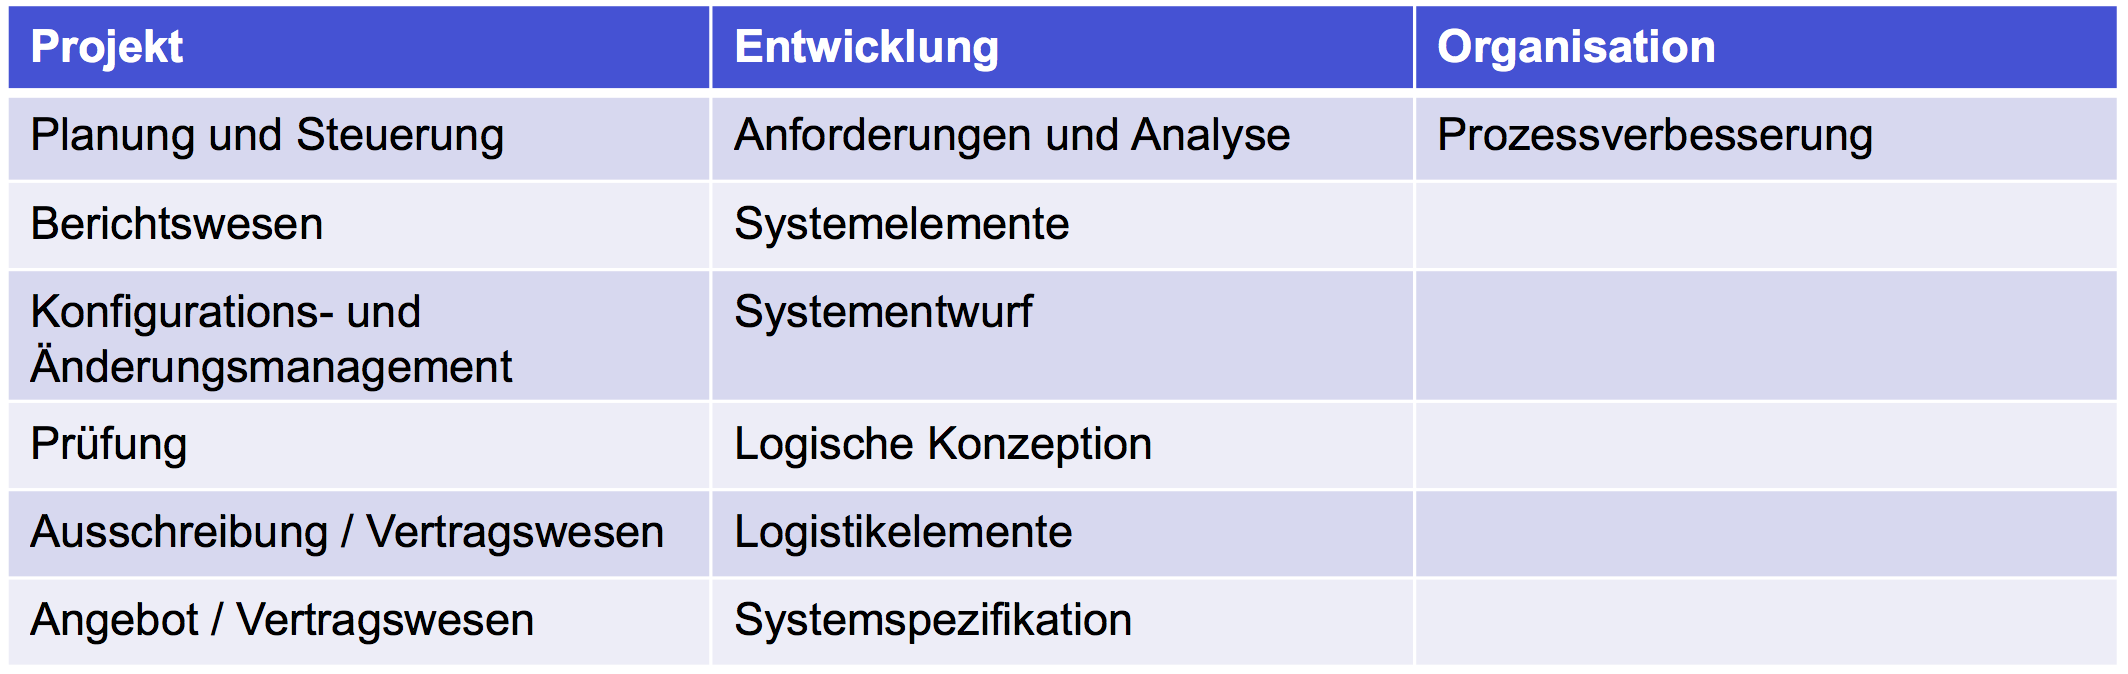
\includegraphics[width=1\textwidth,
			keepaspectratio=true]{bilder/vmodell_disziplinen.png}
\end{frame}

\begin{frame}
\frametitle{V-Modell Xtreme Tailoring}
	\begin{table}
		\caption{Aktivitäten der Disziplin ``Planung und Steuerung''}
		\begin{tabular}{l}
				Planung und Steuerung\\ \hline
				Projektfortschrittsentscheidung herbeiführen \\
				Projekthandbuch erstellen \\
				QS Handbuch erstellen \\
				PM-Infrastruktur einrichten \\
				Schätzung durchführen \\
				Risiken managen \\
				Projekt planen \\
				Arbeitsauftrag vergeben \\
				Kaufm. Projektkalkulation durchführen
		\end{tabular}
	\end{table}
\end{frame}

\begin{frame}
\frametitle{V-Modell Xtreme Tailoring}
	\center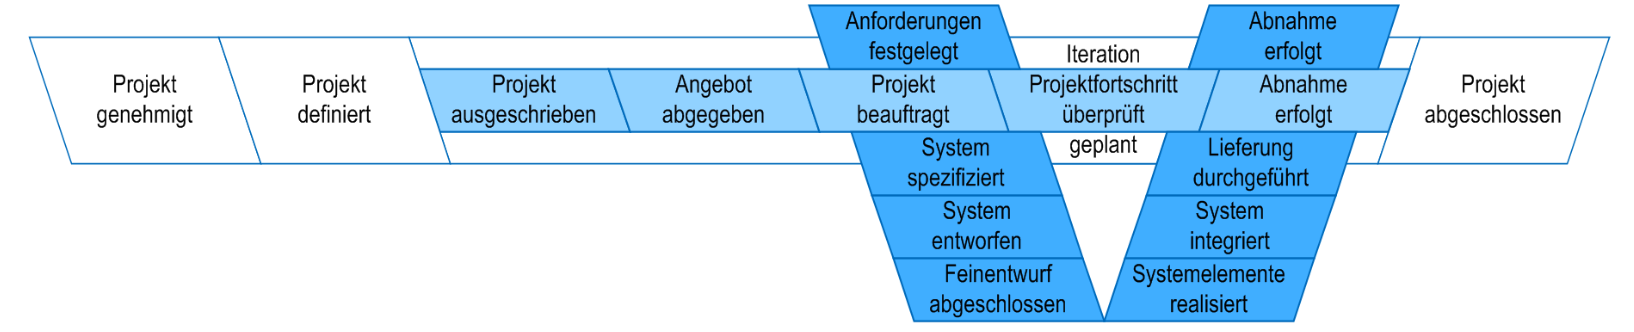
\includegraphics[width=1\textwidth,
			keepaspectratio=true]{bilder/vmodell_xt.png}
	\begin{itemize}
		\item Managementaspekte (weiße Entscheidungspunkte) sind in jeder Projektdurchführungsstrategie enthalten
		\item Auftraggeber-/Auftragnehmer-Schnittstelle (hellblaue Entscheidungspunkte) betreffen die Schnittstelle
		zwischen Auftraggeber und Auftragnehmerprojekten
		\item Systemerstellung (dunkelblaue Entscheidungspunkte) beziehen sich auf die Systemerstellung
	\end{itemize}
\end{frame}

\begin{frame}
\frametitle{V-Modell Xtreme Tailoring}
	\begin{itemize}
		\item V-Modell XT wird aus Vorgehensbausteinen zusammen gesetzt
		\item Vorgehensbaustein fasst die für konkrete Aufgabe erforderlichen
					Disziplinen zusammen (z.B. alle Disziplinen die für Änderungsmanagement)
		\item Auch die an Produkt mitwirkenden Rollen werden durch Vorgehensbaustein
					festgelegt
		\item Den V-Modell Kern bilden folgende Bausteine:
					\begin{itemize}
						\item Projektmanagement
						\item Qualitätssicherung
						\item Problem- und Änderungsmanagement
						\item Konfigurationsmanagement
					\end{itemize}
	 \item Abhängig von Projektmerkmalen kommen weitere Bausteine dazu
	\end{itemize}
\end{frame}

\begin{frame}
\frametitle{V-Modell}
	Vorteile
	\begin{itemize}
		\item Öffentlich zugänglich
		\item Werkzeuge und Dokumentation existieren
		\item V-Modell XT kann als Baukasten verwendet und an Projektsituation angepasst werden
		\item Enthält viele Produktvorlagen
	\end{itemize}
	\bigskip
	Nachteile
	\begin{itemize}
		\item Hohe Komplexität erfordert hohen Schulungsaufwand
		\item Generiert hohe Menge an Artefakten
		\item Managementaufwand ist hoch
	\end{itemize}
\end{frame}

\subsection{Agile Prozessmodelle}
\begin{frame}
\frametitle{Agile Prozessmodelle}
\huge Agile Prozessmodelle
\end{frame}

\begin{frame}
\frametitle{Agile Prozessmodelle}
	\begin{block}{Agil}
		\begin{itemize}
			\item Prozessmodell mit kleinem bis mittlerem Umfang beschrieben
			\item Geringer Aufwand für Dokumentation
			\item Flexible Prozessabläufe
			\item Teammitglieder, Kunde, Code liegen im Fokus
		\end{itemize}
	\end{block}
\end{frame}

\begin{frame}
\frametitle{Agile Manifesto}
	\begin{block}{Agiles Manifest}
		\begin{itemize}
			\item Einzelpersonen und Interaktion \textgreater Prozesse und Werkzeuge
			\item Laufende Systeme \textgreater Umfassende Dokumentation
			\item Zusammenarbeit mit Kunden \textgreater Vertragsverhandlungen
			\item Reaktion auf Änderung \textgreater Verfolgen eines Plans
		\end{itemize}
	\end{block}
\end{frame}

\begin{frame}
\frametitle{Extreme Programming}
	\begin{itemize}
		\item Formale Aspekte der SW werden auf Minimum reduziert
					\begin{itemize}
						\item Verzicht auf Dokumentation
						\item Fokus auf lauffähigen Code
					\end{itemize}
		\item Statt auf detailliertem Prozessmodell basiert XP auf
					\begin{itemize}
						\item Werten
						\item Prinzipien
						\item Praktiken
					\end{itemize}
		\item Testfälle (Modul- und Akzeptanztests) ersetzen Spezifikation und Entwurf
	\end{itemize}
\end{frame}

\begin{frame}
\frametitle{Extreme Programming}
	Werte
	\begin{itemize}
		\item Einfachheit: Einfache Lösungen die leicht zu verstehen und schnell zu realisieren sind.
		\item Kommunikation: Persönlich und direkt, Dokumente für Informationsaustausch zweitrangig
		\item Feedback: Schnelle Rückmeldung über Ergebnisse an das Team
		\item Mut: Zur Lücke und zur Kommunikation
	\end{itemize}
\end{frame}

\begin{frame}
\frametitle{Extreme Programming}
	Prinzipien
	\begin{itemize}
		\item Unmittelbares Feedback
		\item Einfachheit anstreben
		\item Inkrementelle Veränderung
		\item Veränderung wollen
		\item Qualitätsarbeit
		\item Lernen lehren
		\item Geringe Anfangsinvestition
		\item Auf Sieg spielen
	\end{itemize}
\end{frame}

\begin{frame}
\frametitle{Extreme Programming}
	\begin{itemize}
		\item Gezielte Experimente
		\item Offene, aufrichtige Kommunikation
		\item Instinkte der Teammitglieder nutzen und nicht dagegen arbeiten
		\item Verantwortung übernehmen
		\item An Projektgegebenheiten anpassen
		\item Mit leichtem Gepäck reisen
		\item Ehrliches Messen
	\end{itemize}
\end{frame}

\begin{frame}
\frametitle{Extreme Programming}
	Praktiken
	\begin{itemize}
		\item Kunde ist Teil des Teams und vor Ort
		\item User Stories
		\item Kurze Releasezyklen
		\item Akzeptanztests
		\item Pair Programming
		\item Testgetriebene Entwicklung
		\item Gemeinsame Verantwortung
	\end{itemize}
\end{frame}

\begin{frame}
\frametitle{Extreme Programming}
	\begin{itemize}
		\item Continuous Integration
		\item Nachhaltiges Tempo
		\item Offene Räume
		\item Planungsspiel
		\item Einfacher Entwurf
		\item Refactoring
		\item Metapher
	\end{itemize}
\end{frame}

\begin{frame}
\frametitle{Xtreme Programming}
	Vorteile
	\begin{itemize}
		\item Testgetrieben
		\item Kundennah
		\item Dokumentation besteht aus Code + User Stories und ist damit offen für Änderungen
		\item Paarweises Programmieren
	\end{itemize}
	\bigskip
	Nachteile
	\begin{itemize}
		\item Wiederverwendung oft nicht gegeben da sehr projekspezifischer Code
		\item Hochqualifizierte Teams gefordert
		\item Sehr hoher Anspruch an Kommunikation
	\end{itemize}
\end{frame}

\begin{frame}
\frametitle{Scrum}
	\begin{itemize}
		\item Managementkonzept dass nicht nur auf SW-Entwicklung beschränkt ist
		\item Setzt auf Selbstorganisation der Entwickler
		\item Ansatz ist empirisch, inkrementell und iterativ
		\item Basiert auf Transparenz, Überprüfung, Anpassung
		\item Vorgehensmodell wird durch wenige einfache Regeln defniert (easy to learn, hard to master)
	\end{itemize}
\end{frame}

\begin{frame}
\frametitle{Scrum}
	Als agiler Prozess kommt Scrum mit einigen wenigen Dokumenten/Artefakten aus (nach Scrum Guide)
	\begin{itemize}
		\item Product Backlog, enthält alle Anforderungen in Form von User Stories nach Priorität absteigeng geordnet
		\item Sprint Backlog, enthält alle Anforderungen in Form von User Stories die im Sprint umgesetzt werden
		\item Inkrement, fertiges Produkt als Sprintergebniss
		\item Definition of Done, gemeinsames Verständnis darüber was es heißt eine Story abgeschlossen zu haben
	\end{itemize}
	Daneben existieren außerdem Sprint Ziele, Burndown Charts, Impediment Backlog, Epic Board \ldots
\end{frame}

\begin{frame}
\frametitle{Scrum}
	Scrum definiert drei Rollen
	\begin{itemize}
		\item Product Ownder
			\begin{itemize}
				\item Kennt fachliche und technische Anforderungen
				\item Pflegt, erweitert und priorisiert das Product Backlog
				\item Beurteilt die Sprintergebnisse
				\item Entwickelt das Produkt weiter, hat eine klare Vision
			\end{itemize}
		\item Scrum Master
			\begin{itemize}
				\item Moderator, Coach, Serving Leader
				\item Sorgt für die Einhaltung der Scrum-Regeln
				\item Hilft bei methodischen Problemen
				\item Beseitigt Hindernisse
				\item Treibt agile Vorgehensweise über Projektgrenzen hinaus voran
			\end{itemize}
		\item Projekt Team
			\begin{itemize}
				\item 4-12 Teammitglieder
				\item Organisiert sich selbst
				\item Keine Hierarchien
				\item Kennt nur Entwickler
				\item Unterschiedliche Kompetenzen
			\end{itemize}
	\end{itemize}
\end{frame}

\begin{frame}
\frametitle{Scrum}
	Scrum definiert eine Reihe von Events
	\begin{itemize}
		\item Daily Scrum, 15 Minuten, 3 Fragen: Was habe ich gestern gemacht? Was mache ich heute? Was blockt mich?
		\item Sprint Review, Vorstellung der Sprintergebnisse
		\item Sprint Retrospective, Reflektion des Sprints, was lief gut, was schlecht
		\item Sprint Planning, erstellen des Sprint-Backlogs, was wird wie erreicht
	\end{itemize}
\end{frame}

\begin{frame}
\frametitle{Scrum}
	\center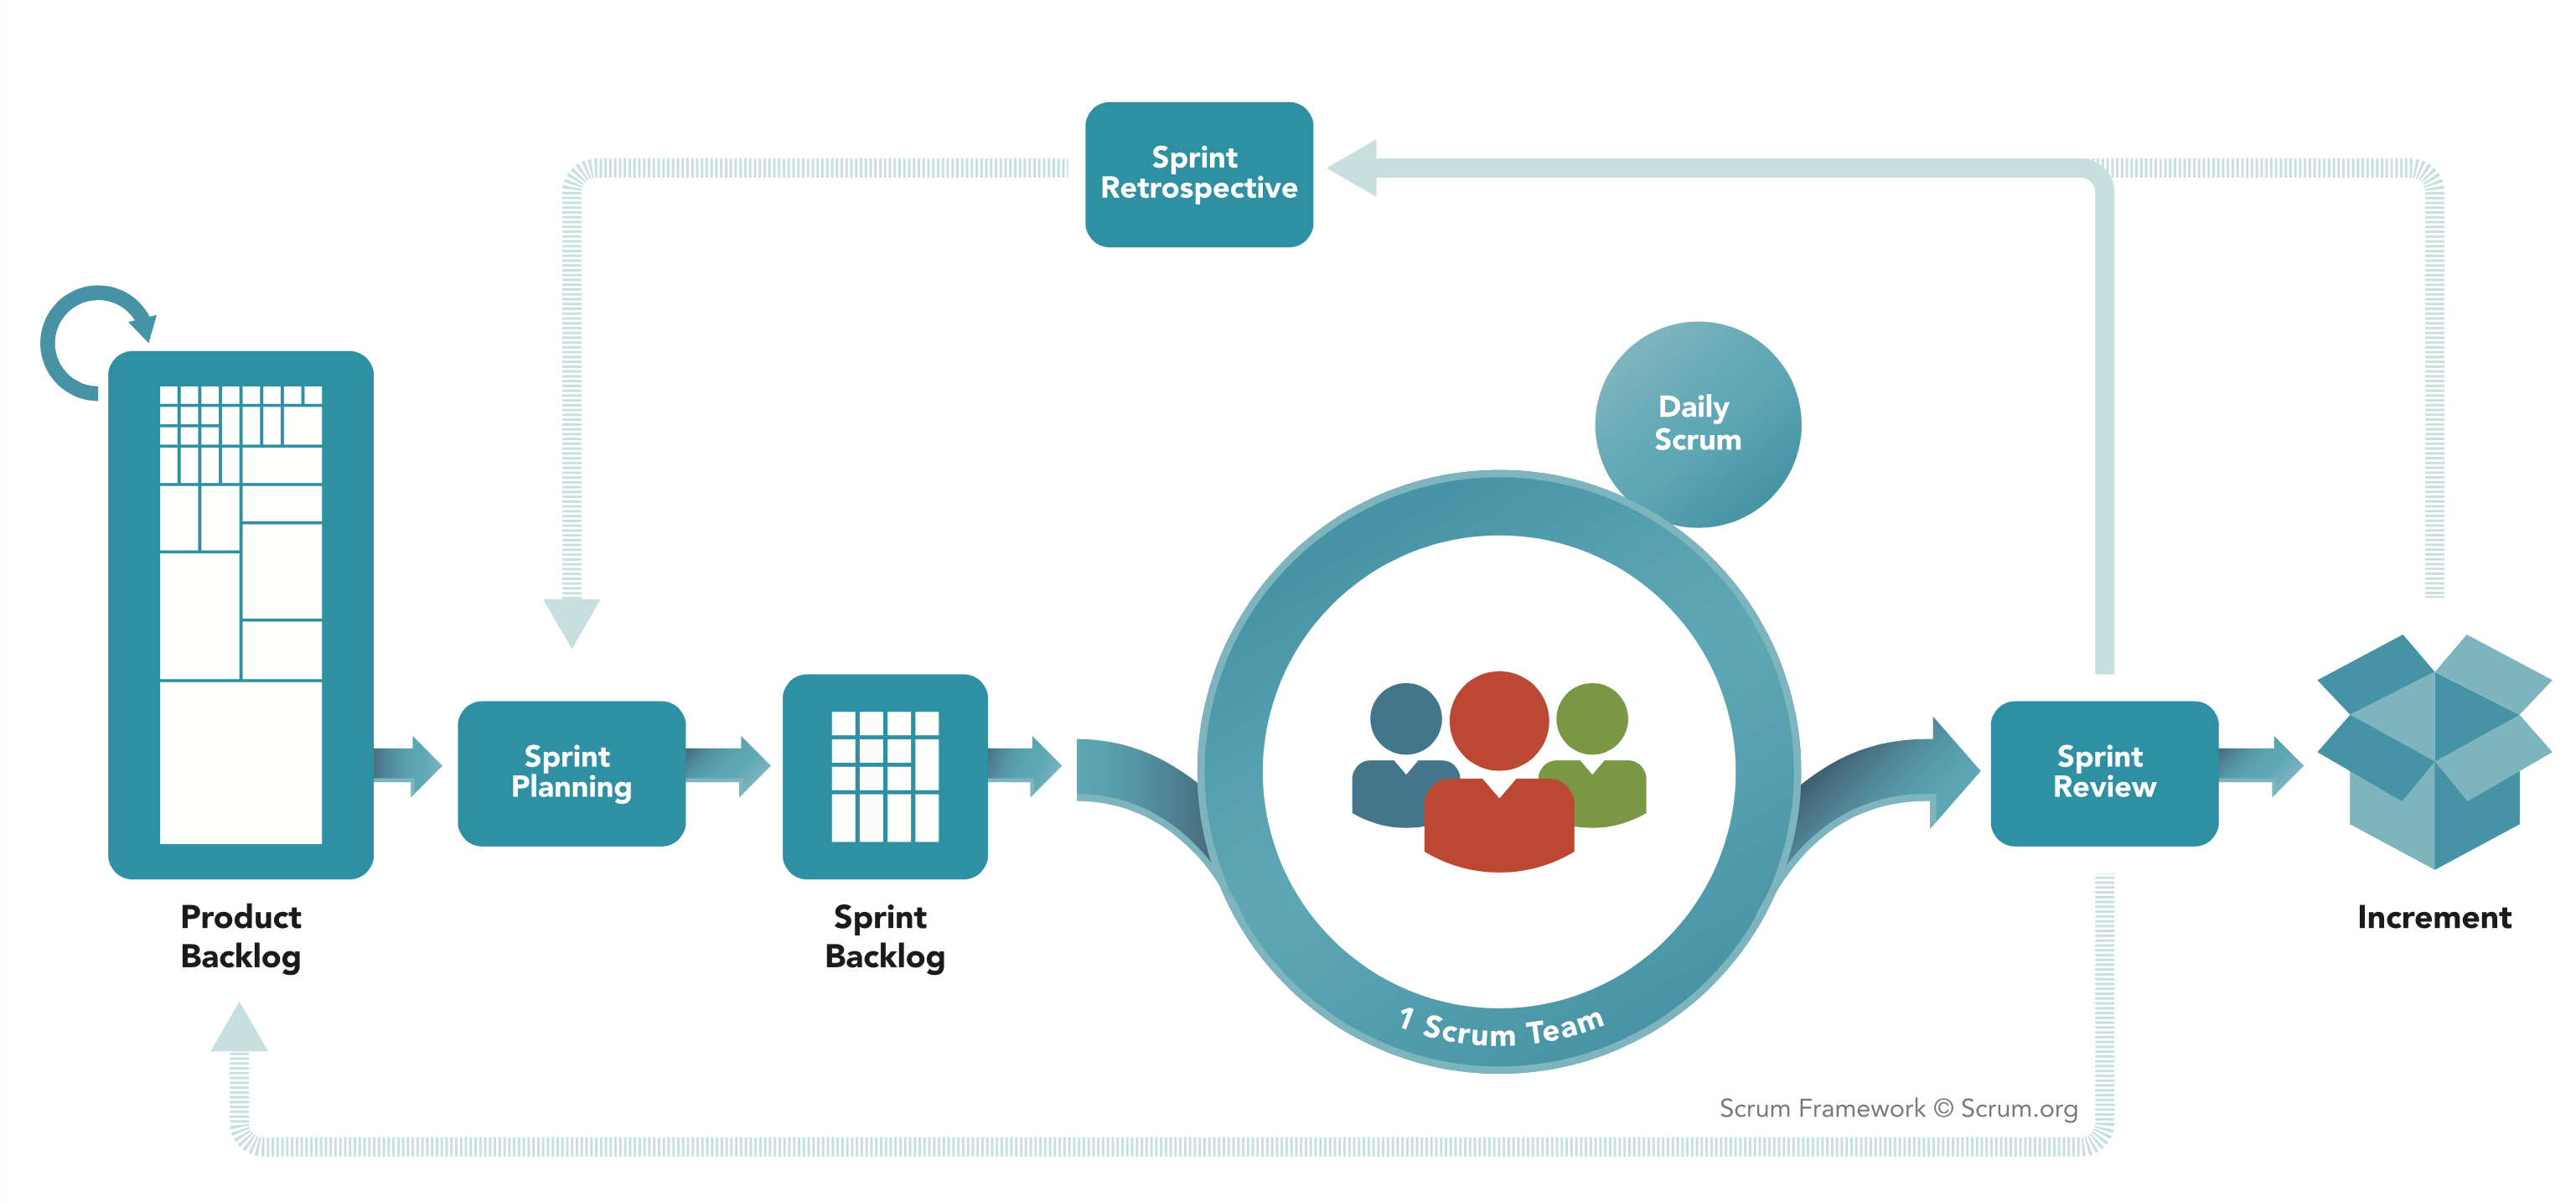
\includegraphics[width=1\textwidth,
		keepaspectratio=true]{bilder/scrum.png}
\end{frame}

\begin{frame}
\frametitle{Scrum}
	Vorteile
	\begin{itemize}
		\item Leichtgewichtig
		\item Klar defnierte Regeln und Abläufe
		\item Fördert Kreativität durch selbstorganisierte Teams
		\item Leicht zu lernen
	\end{itemize}
	\bigskip
	Nachteile
	\begin{itemize}
		\item Wiederverwendung oft nicht gegeben da sehr projekspezifischer Code
		\item Schwierig wenn Teams weltweit verteilt
		\item Regelwerk ist unflexibel
		\item Schwer zu meistern
	\end{itemize}
\end{frame}

\begin{frame}
\frametitle{Kanban}
	Kanban definiert sich durch vier Elemente
	\begin{itemize}
		\item Arbeit wird genommen, nicht gegeben
		\item Mengen werden limitiert
		\item Informationen werden veröffentlicht
		\item Abläufe werden kontinuierlich verbessert
	\end{itemize}
\end{frame}

\begin{frame}
\frametitle{Kanban}
	\begin{itemize}
		\item Kanban-Board ist zentrales Element
		\item Besteht aus frei definierbaren Spalten
		\item Visualisiert den Entwicklungsprozess
		\item User-Stories/Arbeitspakete werden eigenständig vom Team dem Prozess nach abgearbeitet
		\item Wann eine einzelnen Phase abgeschlossen ist wird in der Definition of Done festgelegt
		\item Jede Phase hat ein Limit das die maximale Anzahl aufgenommener Aufgaben angibt
		\item Limit macht Engpässe transparent
	\end{itemize}
\end{frame}

\begin{frame}
\frametitle{Kanban}
\center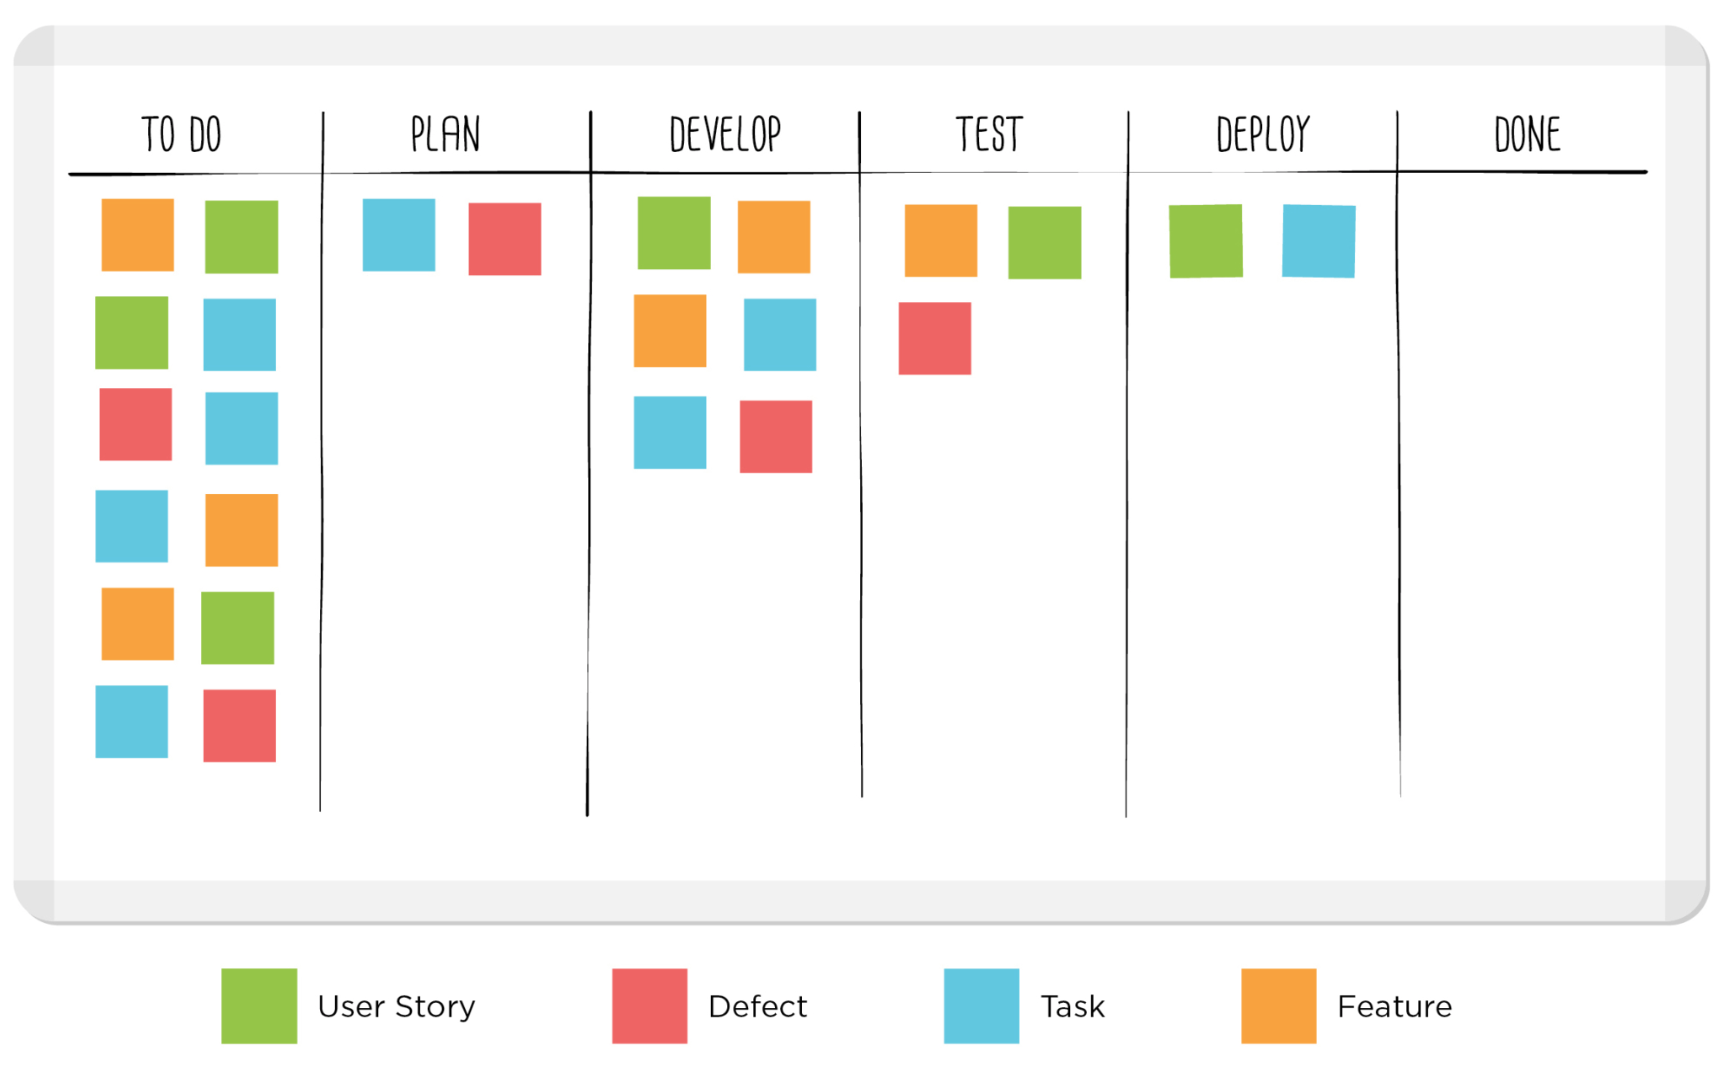
\includegraphics[width=1\textwidth,
	keepaspectratio=true]{bilder/kanban_board.png}
\end{frame}

\begin{frame}
\frametitle{Kanban}
	Metriken dienen als Grundlage der kontinuierlichen Verbesserung
	\begin{itemize}
		\item Cumulative Flow Diagram = Summe aller Aufgaben pro Phase in Abhängigkeit der Zeit
		\item Anzahl der Tickets die Work-in-Progress sind
		\item Durchsatz an Tickets pro Woche
		\item Durchschnittliche Zeit die ein Ticket für gesamten Durchlauf benötigt
	\end{itemize}
\end{frame}

\begin{frame}
\frametitle{Kanban}
	Vorteile
	\begin{itemize}
		\item Leichtgewichtig
		\item Sehr leicht zu lernen
		\item Forciert einen ausgeglichenen Arbeitsfluss
		\item Probleme werden direkt visualisiert
	\end{itemize}
	\bigskip
	Nachteile
	\begin{itemize}
		\item Für große Projekte unübersichtlich
		\item Nicht auf Einzelprojekte/Neuprojekte anwendbar
	\end{itemize}
\end{frame}
